\documentclass[11pt,letterpaper]{article}
\usepackage[utf8]{inputenc}
\usepackage[T1]{fontenc}
\usepackage{lmodern}
\usepackage[DIV=11]{typearea} 

\usepackage{todonotes}
\usepackage{microtype}

\usepackage{amssymb}
\usepackage{amsmath}
\usepackage{amsthm}
\usepackage[basic]{complexity}
\usepackage{thmtools}
\usepackage[ruled,vlined,linesnumbered,nokwfunc]{algorithm2e_}

\usepackage{tikz}
\usetikzlibrary{arrows,shapes}
\usetikzlibrary{decorations,shadows}
\tikzstyle{player}=[draw, thick, circle, fill=gray!15,inner sep=2pt, minimum width=12pt]
\tikzstyle{vplayer}=[draw, thick, circle, fill=gray!15,inner sep=0.5pt, minimum width=12pt]
\tikzstyle{random}=[draw, thick, diamond, rounded corners, fill=gray!15,inner sep=2pt, minimum width=12pt]
\tikzstyle{vrandom}=[draw, thick, diamond, rounded corners, fill=gray!15,inner sep=0.5pt, minimum width=12pt]

\usepackage{xcolor}
\usepackage{xspace}
\usepackage{paralist}
\usepackage{booktabs}
\usepackage{multirow}

\makeatletter
\newsavebox{\@brx}
\newcommand{\llangle}[1][]{\savebox{\@brx}{}\mathopen{\copy\@brx\mkern2mu\kern-0.9\wd\@brx\usebox{\@brx}}}
\newcommand{\rrangle}[1][]{\savebox{\@brx}{}\mathclose{\copy\@brx\mkern2mu\kern-0.9\wd\@brx\usebox{\@brx}}}
\makeatother
\newcommand{\as}[1]{\llangle 1 \rrangle_\textit{as}\left(#1\right)}
\newcommand*{\ditto}{---\textquotedbl---} 

\newcommand{\set}[1]{\{#1\}}
\newcommand{\lu}{\textup{(}}
\newcommand{\ru}{\textup{)}\xspace}
\newcommand{\upbr}[1]{\lu #1\ru}

\newcommand{\at}{\mathit{Attr}}
\newcommand{\ate}{\mathit{Attr}^+}
\newcommand{\Inf}{\mathrm{Inf}}
\newcommand{\pr}[3]{\mathrm{Pr}^{#1}_{#2}\left(#3\right)}
\newcommand{\reacht}[1]{\textrm{Reach}\left(#1\right)}
\newcommand{\streett}[1]{\textrm{Streett}\left(#1\right)}
\newcommand{\objsty}[2]{\textrm{#1}\left(#2\right)}
\newcommand{\SP}{\mathrm{SP}}
\renewcommand{\RP}{\mathrm{RP}}

\newcommand{\pat}{\omega\xspace}
\newcommand{\Path}{\Omega\xspace}
\newcommand{\str}{\sigma\xspace}
\newcommand{\Str}{\Sigma\xspace}
\newcommand{\obj}{\psi\xspace}
\newcommand{\sseq}{\langle v_0,v_1,v_2,\ldots\rangle}

\newcommand{\mdp}{P\xspace}
\newcommand{\vo}{V_1\xspace}
\newcommand{\vr}{V_R\xspace}
\newcommand{\trans}{\delta\xspace}
\newcommand{\target}{T\xspace}
\newcommand{\intarget}{\expandafter\MakeLowercase\expandafter{\target}\xspace}
\newcommand{\ec}{X\xspace}
\newcommand{\inec}{\expandafter\MakeLowercase\expandafter{\ec}\xspace}
\newcommand{\scc}{C\xspace}
\newcommand{\inscc}{\expandafter\MakeLowercase\expandafter{\scc}\xspace}

\newcommand{\mecalg}{\ProcNameSty{allMECs}}
\newcommand{\allsccalg}{\ProcNameSty{SCCs}}
\newcommand{\sccalg}{\ProcNameSty{SmallestBSCC}}
\newcommand{\reach}{\ProcNameSty{GraphReach}}
\newcommand{\good}{\DataSty{goodEC}}
\newcommand{\winning}{\DataSty{winMEC}}
\newcommand{\badv}{B\xspace}
\newcommand{\rev}{\mathit{RevG}}
\newcommand{\blue}{\mathit{Bl}}
\newcommand{\Out}{\mathit{Out}}
\newcommand{\In}{\mathit{In}}
\newcommand{\OutDeg}{\mathit{Outdeg}}
\newcommand{\InDeg}{\mathit{Indeg}}

\newcommand{\remove}{\ProcNameSty{Remove}}
\newcommand{\bad}{\ProcNameSty{Bad}}
\newcommand{\construct}{\ProcNameSty{Construct}}
\newcommand{\bits}{\mathit{bits}\xspace}
\newcommand{\ds}{\mathit{D}\xspace}


\newif\iffullversion
\newcommand{\infull}[1]{\iffullversion #1\fi}
\newcommand{\inshort}[1]{\iffullversion \else #1\fi}

\fullversiontrue

\declaretheorem[numberwithin=section]{theorem}
\declaretheorem[numberlike=theorem]{lemma}
\declaretheorem[numberlike=theorem]{proposition}
\declaretheorem[numberlike=theorem]{corollary}
\declaretheorem[numberlike=theorem]{definition}
\declaretheorem[numberlike=theorem]{observation}
\declaretheorem[numbered=no,name=Observation]{observation*}
\declaretheorem[numberlike=theorem]{reduction}
\declaretheorem[numberlike=theorem]{conjecture}
\declaretheorem[numberlike=theorem]{invariant}
\declaretheorem[numberlike=theorem]{remark}

\DontPrintSemicolon
\SetAlCapFnt{\normalfont\scshape}
\SetProcNameSty{texttt}
\SetFuncSty{texttt}

\usepackage{authblk}

\begin{document}
\title{Model and Objective Separation with Conditional Lower Bounds: Disjunction is Harder than Conjunction}
\author[1]{Krishnendu Chatterjee}
\affil[1]{IST Austria}
\author[2]{Wolfgang Dvo{\v r}{\' a}k}
\author[2]{Monika Henzinger}
\author[2]{Veronika~Loitzenbauer}
\affil[2]{University of Vienna, Faculty of Computer Science}

\maketitle

\begin{abstract}
Given a model of a system and an objective, the model-checking question asks 
whether the model satisfies the objective. We study polynomial-time problems in 
two classical models, graphs and Markov Decision Processes (MDPs), with respect to 
several fundamental -regular objectives, e.g., Rabin and Streett objectives. 
For many of these problems the best-known upper bounds are quadratic or cubic, 
yet no super-linear lower bounds are known. 
In this work our contributions are two-fold: First, we present several improved 
algorithms, and second, we present the first conditional super-linear lower bounds 
based on widely believed assumptions about the complexity of CNF-SAT and combinatorial Boolean 
matrix multiplication. 
A separation result for two models with respect to an objective means a conditional 
lower bound for one model that is strictly higher than the existing upper bound 
for the other model, and similarly for two objectives with respect to a model. 
Our results establish the following separation results: 
(1) A separation of models (graphs and MDPs) for disjunctive queries of 
reachability and B\"uchi objectives.
(2) Two kinds of separations of objectives, both for graphs and MDPs, namely, 
(2a) the separation of dual objectives such as \infull{reachability/safety (for 
disjunctive questions) and }Streett/Rabin objectives, and (2b) the separation of
conjunction and disjunction of multiple objectives of the same type such as safety, B\"uchi, and coB\"uchi. 
In summary, our results establish the first model and objective separation 
results for graphs and MDPs for various classical -regular objectives. 
Quite strikingly, we establish conditional lower bounds for the disjunction of
objectives that are strictly higher than the existing upper bounds for the 
conjunction of the same objectives.

\end{abstract}

\section{Introduction}
The fundamental problem in formal verification is the \emph{model-checking} 
question that given a model of a system and a property asks whether the model 
satisfies the property. 
The model can be, for example, a standard graph, or a probabilistic extension of 
graphs, and the property describes the desired behaviors\infull{ (or infinite paths)}
of the model. 
For several basic model-checking questions, though polynomial-time 
algorithms are known, the best-known existing upper bounds are quadratic or 
cubic, yet no super-linear lower bounds are known.
In graph algorithmic problems unconditional super-linear lower bounds are very 
rare when polynomial-time solutions exist.
However, recently there have been many interesting results that establish 
\emph{conditional lower bounds}~\cite{AbboudW14,AbboudWY15,AbboudBW15a}.
These are lower bounds based on the assumption that 
for some well-studied problem such as 3-SUM~\cite{GajentaanO12} or All-Pairs 
Shortest Paths~\cite{WilliamsW10,RodittyZ11} no (polynomially\footnote{In particular
improvements by polylogarithmic factors are not excluded.}) faster algorithm 
exists (compared to the best known algorithm).
The lower bounds in this work assume
(A1)~there is no combinatorial\footnote{Combinatorial here means avoiding fast matrix multiplication~\cite{LeGall14}, see also the 
discussion in~\cite{HenzingerKNS15}.} algorithm with running time of
 for any 
to multiply two  Boolean matrices;
or (A2)~for all  there exists a  such that there is no algorithm 
for the -CNF-SAT problem that runs in  time, where  is the number of variables and  the number of clauses. 
These two assumptions have been used to establish lower bounds for 
several well-studied problems, such as dynamic graph algorithms~\cite{AbboudW14,AbboudWY15}, 
measuring the similarity of strings~\cite{AbboudWW14,Bringmann14,
BringmannK15,BackursI15,AbboudBW15b}, context-free grammar
parsing~\cite{Lee02,AbboudBW15a}, and verifying first-order graph 
properties~\cite{PatrascuW10,Williams14}. 
No relation between conjectures (A1) and (A2) is known. 
In this work we present conditional lower bounds that are super-linear 
for fundamental model-checking problems.

\smallskip\noindent{\em Models.} 
The two most classical models in formal verification are 
\emph{standard graphs} and \emph{Markov decision processes \upbr{MDPs}}. 
MDPs are probabilistic extensions of graphs, 
and an MDP consists of a finite 
directed graph  with a partition of the vertex set~ into 
player~1 vertices  and random vertices 
and a probabilistic transition function that specifies for vertices in 
a probability distribution over their successor vertices. 
Let  and . 
An infinite path in an MDP is obtained by the following process. 
A token is placed on an initial vertex and the token is moved indefinitely 
as follows: At a vertex  a choice is made to move the token along 
one of the outedges of~, and at a vertex  the token is moved 
according to the probabilistic transition function. 
Note that if , then we have a standard graph, and 
if , then we have a Markov chain.
Thus MDPs generalize standard graphs and Markov chains.

\smallskip\noindent{\em Objectives.}
Objectives (or properties) are subsets of infinite paths that specify the 
desired set of paths. \inshort{Let  be a set of target
vertices.}
The most basic objective is \emph{reachability} where\infull{, given a set 
 of \emph{target} vertices,} an infinite path satisfies the 
objective if the path visits a vertex of  {\em at least once}.
The dual objective to reachability is \emph{safety} where\infull{, given a set 
 of \emph{target} vertices,} an infinite path satisfies the 
objective if the path does \emph{not} visit any vertex of .
The next extension of a reachability objective is the 
\emph{Büchi} objective that requires the set\infull{ of target vertices}\inshort{~} 
to be reached \emph{infinitely often}. Its dual, the \emph{coBüchi} objective, 
requires the set\infull{ of target vertices}\inshort{~} to be reached only \emph{finitely often}.
A natural extension of single objectives are \emph{conjunctive} and \emph{disjunctive} 
\emph{objectives}~\cite{FijalkowH12,Wolper00,ChatterjeeHP07}. For two objectives
 and  their conjunctive objective is equal to 
and their disjunctive objective is equal to .
The conjunction of reachability (resp.\ Büchi) objectives is known as 
\emph{generalized reachability \upbr{resp.\ Büchi}}~\cite{FijalkowH12,Wolper00}.
A very central and canonical class of objectives in formal verification are 
\emph{Streett} (strong fairness) objectives and their dual \emph{Rabin} objectives~\cite{Thomas97}.
A \emph{one-pair Streett} objective for two sets of vertices  and  specifies
that if the Büchi objective for target set  is satisfied, then also the Büchi
objective for target set  has to be satisfied; in other words, a one-pair 
Streett objective is the disjunction of a coBüchi objective (with target set 
) and a Büchi objective (with target set ).
The dual \emph{one-pair Rabin} objective for two vertex sets  and  
is the conjunction of a Büchi objective with target set  and a
coBüchi objective with target set .
A Streett objective is the conjunction of  one-pair Streett objectives
and its dual Rabin objective is the disjunction of  one-pair Rabin objectives.

\smallskip\noindent{\em Algorithmic questions.}
\infull{The algorithmic question given a model and an objective is as follows: 
(a)~for standard graphs, the model-checking question asks whether there is a 
path that satisfies the objective; and 
(b)~for MDPs, the basic model-checking question asks 
}
\inshort{Given a model and an objective, the algorithmic question 
(a)~for standard graphs is whether there is a path that satisfies
the objective and (b)~for MDPs is}
whether there is a 
\infull{\emph{policy} (or a }\emph{strategy} that resolves the 
non-deterministic choices of outgoing 
edges\infull{)} for player~1 to ensure that the objective is satisfied with 
probability~1.
Observe that if we consider the model-checking question for MDPs with 
, then it exactly corresponds to the model-checking question 
for standard graphs.
Given  objectives, the \emph{conjunctive query} question asks whether
there is a \infull{policy}\inshort{strategy} for player~1 to ensure that \emph{all}
the objectives 
are satisfied with probability~1, and the \emph{disjunctive query}
question asks whether there is a \infull{policy}\inshort{strategy} for player~1 to ensure that \emph{one}
of the objectives is satisfied with probability~1.
Conjunctive queries coincide with conjunctive objectives on graphs and MDPs,
while disjunctive queries coincide with disjunctive objectives on graphs but not MDPs\infull{ (see 
Observations~\ref{obs:conj} and~\ref{obs:disjgraph})}.

\smallskip\noindent{\em Significance of model and objectives.} 
Standard graphs are the model for non-deterministic systems, and provide the 
framework to model hardware and software systems~\cite{SPIN,NUSMV}, as well
as many basic logic-related questions such as automata emptiness. 
MDPs model systems with both non-deterministic and probabilistic behavior; 
and provide the framework for a wide range of applications from randomized 
communication and security protocols, to stochastic distributed systems, 
to biological systems~\cite{prism,baierbook}.
In verification, reachability objectives are the most basic objectives for 
safety-critical systems.
In general all properties that arise in verification (such as liveness, 
fairness) are -regular languages (-regular languages extend 
regular languages to infinite words), and every -regular language can 
be expressed as a Streett objective (or a Rabin objective). Important special
cases of Streett (resp.\ Rabin) objectives are Büchi and coBüchi objectives~\cite{ChatterjeeH14}.
Thus the algorithmic questions we consider are the most basic questions in 
formal verification.

\smallskip\noindent{\em Model separation and objective separation questions.} 
In this work our results (upper and conditional lower bounds) aim to establish 
the following two fundamental separations:

\begin{itemize}
\item {\em Model separation.} 
Consider an objective where the algorithmic question for both graphs and MDPs 
can be solved in polynomial time, and establish a conditional lower bound for 
MDPs that is strictly higher than the best-known upper bound for graphs. 
\infull{In other words, the conditional lower bound would separate the model of 
graphs and MDPs for problems (i.e., w.r.t.\ the objective) that can be solved in 
polynomial time.}

\item {\em Objective separation.} 
Consider a model (either graphs or MDPs) with two different objectives and 
show that, though the algorithmic question for both objectives can be solved in 
polynomial time, there is a conditional lower bound for one objective that 
is strictly higher than the best-known upper bound for the other objective.
\infull{In other words, the conditional lower bound would separate the two objectives 
w.r.t.\ the model though they both can be solved in polynomial time.}
\end{itemize}
To the best of our knowledge, there is no previous work that establish any 
model separation or objective separation result in the literature.

\smallskip\noindent{\em Our results.} 
In this work we present improved algorithms as well as 
the first conditional lower bounds that are super-linear for algorithmic 
problems in model checking that can be solved in polynomial time, and together
they establish both model separation and objective separation results. 
An overview of the results for the different objectives is given in Table~\ref{tab:comparison},
where our results are highlighted in boldface.
We use  
\textsc{MEC} to refer to the time to compute the maximal end-component 
decomposition of an MDP. An end-component is a\infull{ (non-trivial)}
strongly connected sub-MDP
that has no outgoing edges for random vertices. We have ~\cite{ChatterjeeH14}\infull{ and assume  
and }.
Moreover, we use 
 to denote the number of combined objectives in the case of conjunction 
or disjunction of multiple objectives and 
 to denote the total number of elements in all the target sets
that specify the objectives.
We first describe Table~\ref{tab:comparison} and our main results and then 
discuss the significance of our results for model and objective separation.

\begin{table*}[!t]
\renewcommand{\arraystretch}{1.3}
\inshort{\nocaptionrule} \caption{Upper and lower bounds.
Our results are boldface and respective results are referred.}\label{tab:comparison}
\centering
\small\scriptsize
\begin{tabular}{@{}*{2}{l}*{4}{c}@{}}
\toprule
 &  & \multicolumn{2}{c}{Graphs} & \multicolumn{2}{c}{MDPs} \\
\cmidrule{3-4}\cmidrule{5-6}
& & upper bound & lower bound & upper bound & lower bound \\
\midrule
Reach & Conj. & \multicolumn{2}{c}{\NP-c~\cite{ChatterjeeAM13}}\phantom{abcdef} & \multicolumn{2}{c}{\PSPACE-c~\cite{FijalkowH12}} \\
\cmidrule{2-6}
& Disj.\ Obj. & \multicolumn{2}{c}{\multirow{2}{*}{\phantom{abcdef}}}  
& ~\cite{ChatterjeeJH03,ChatterjeeH14} \\
& Disj.\ Qu. & \multicolumn{2}{c}{} &  \inshort{[Th.~\ref{thm:reach_alg}]} & 
 \inshort{[Th.~\ref{thm:reach_STChard}]},  \inshort{[Th.~\ref{thm:reach_OVChard}]}\\
\midrule
Safety  & Conj. & \multicolumn{2}{c}{\phantom{abcdef}} & 
\multicolumn{2}{c}{}\\
\cmidrule{2-6}
& Disj.\ Obj. & \multirow{2}{*}{} & 
\multirow{2}{*}{ \inshort{[Th.~\ref{thm:safety_STChard}]}}
& \multicolumn{2}{c}{\PSPACE-c~\cite{FijalkowH12}} \\
& Disj.\ Qu. & & &  &  \inshort{[Th.~\ref{thm:safety_STChard}]},  \inshort{[Th.~\ref{thm:safety_OVChard}]}\\
\midrule
B{\"u}chi  & Conj. & \multicolumn{2}{c}{\phantom{abcdef}} &  \\
\cmidrule{2-6}
& Disj.\ Obj. & \multicolumn{2}{c}{\multirow{2}{*}{\phantom{abcdef}}} 
& ~\cite{ChatterjeeJH03,ChatterjeeH14} \\
& Disj.\ Qu. & \multicolumn{2}{c}{} &  \inshort{[Th.~\ref{thm:reach_alg}]} & 
 \inshort{[Cor.~\ref{cor:STC}]},  \inshort{[Cor.~\ref{cor:OVC}]}\\
\midrule
coB{\"u}chi & Conj. & \multicolumn{2}{c}{\phantom{abcdef}} &  \\
\cmidrule{2-6}
& Disj.\ Obj. & \multirow{2}{*}{} & 
\multirow{2}{*}{ \inshort{[Cor.~\ref{cor:STC}]}}
&  \inshort{[Th.~\ref{thm:cobuchi_alg}]} &  \inshort{[Cor.~\ref{cor:STC}]},  \inshort{[Cor.~\ref{cor:OVC}]}\\
& Disj.\ Qu. & & &  \inshort{[Th.~\ref{thm:cobuchi_alg}]} &  \inshort{[Cor.~\ref{cor:STC}]},  \inshort{[Cor.~\ref{cor:OVC}]}\\
\cmidrule{2-6}
Singleton & Disj.\ Obj.& \multicolumn{2}{c}{\multirow{2}{*}{ \inshort{[Th.~\ref{thm:singleton_alg}]}\phantom{abcdef}}} & &  \inshort{[Cor.~\ref{cor:OVC}]}\\
& Disj.\ Qu. & & & &  \inshort{[Cor.~\ref{cor:OVC}]}\\
\midrule
Streett & & \multicolumn{2}{l}{
\cite{HenzingerT96,ChatterjeeHL15}}
& \multicolumn{2}{l}{ \inshort{[Th.~\ref{thm:streett_alg}]}}\\
\midrule
Rabin & &  & 
 \inshort{[Cor.~\ref{cor:STC}]}
&  & 
 \inshort{[Cor.~\ref{cor:STC}]},  \inshort{[Cor.~\ref{cor:OVC}]}\\
\bottomrule
\multicolumn{6}{l}{  lower bounds  are based on the \inshort{combinatorial Boolean Matrix Multiplication}\infull{BMM} Conjecture / Strong Triangle Conjecture~(A1)
} \\ 
\multicolumn{6}{l}{\phantom{}  lower bounds are based on the Orthogonal Vectors Conjecture
/ Strong ETH~(A2)
}
\end{tabular}
\end{table*}

\begin{enumerate}
\item
\emph{Conjunctive and Disjunctive Reachability \upbr{and Büchi} Problems.} 
    First, we consider conjunctive and disjunctive reachability objectives and 
    queries. Recall that conjunctive objectives and queries in general
    and disjunctive objectives and queries on graphs coincide. For reachability
    further the disjunctive objective can be reduced to a single objective\infull{ (see 
    Observation~\ref{obs:disjobjreach})}.
    The following results are known: the algorithmic question for conjunctive 
    reachability objectives is \NP-complete for 
    graphs~\cite{ChatterjeeAM13}, and \PSPACE-complete for MDPs~\cite{FijalkowH12};
    and the disjunctive objective 
    can be solved in linear time for graphs
    and in  time in MDPs~\cite{ChatterjeeJH03,ChatterjeeH14}.
    We present three results for disjunctive reachability queries in MDPs: 
    (i)~We present an -time algorithm\infull{\footnote{This implies an -time algorithm for disjunctive objective but does not 
    improve the running time for this case.}}.
    (ii)~We show that under assumption (A1) there does not exist a combinatorial
     algorithm for any .
    (iii)~We show that for  
    there does not exist an 
     time algorithm for any  under assumption (A2). 
     Hence we establish an upper bound and matching conditional lower bounds
     based on (A1) and (A2).

		Disjunctive Büchi objectives (on graphs and MDPs) 
		can be reduced in linear time to disjunctive
		reachability objectives and vice versa, therefore 
		the same results apply to disjunctive Büchi problems\infull{ (see Observation~\ref{obs:Reachability_Buchi})}.
		The basic algorithm for conjunctive Büchi objectives runs in time 
		on graphs and in time  on MDPs.
 
\item
\emph{Conjunctive and Disjunctive Safety Problems.}
    Second, we consider conjunctive and disjunctive safety objectives and queries.
    The following results are known: the conjunctive problem can be reduced
    to a single objective and can be solved in linear 
    time, both in graphs and MDPs (see e.g.~\cite{ChatterjeeDH10}); disjunctive queries for MDPs can be solved in  time; and disjunctive objectives for MDPs
    are \PSPACE-complete~\cite{FijalkowH12}.
    We present two results: 
    (i)~We show that for the disjunctive problem in graphs 
    under assumption (A1) there does not exist a combinatorial
     algorithm for any .
    This implies the same conditional lower bound for disjunctive queries
    and objectives in MDPs and matches the upper bound for graphs 
    and disjunctive queries in MDPs.
    (ii)~We present, for ,
    an  lower bound for disjunctive 
    objectives and queries in MDPs under assumption (A2). 
    Again this lower bound matches the upper bound of 
    for disjunctive queries.

\item
\emph{Conjunctive and Disjunctive coBüchi Problems.}
	For coBüchi, a conjunctive objective can be reduced to a single objective.
	For single objectives the basic algorithm runs in time  on MDPs
	and in time  on graphs.
	\infull{Since the conditional lower bounds for disjunctive safety objectives and 
	queries actually already apply for the non-emptiness of the winning set, 
	the reductions also hold for coBüchi (see 
	Observation~\ref{obs:nonempty_safety_coBuchi}).}
	\inshort{Our conditional lower bounds for disjunctive safety objectives and 
	queries also hold for coBüchi objectives.}
	Here the running times and the conditional lower bounds are matching for both
	disjunctive queries and disjunctive objectives.
	For the conditional lower bound based on assumption (A2)
	only \emph{singleton coBüchi} objectives, i.e., coBüchi objectives with target 
	sets of cardinality one, are needed, 
	therefore the bound already holds for this case. 
	We additionally present two results:
	(i)~We present -time algorithms for 
    disjunctive queries and objectives in MDPs.
   (ii)~We present a linear time algorithm for 
   disjunctive singleton coBüchi objectives in graphs.
	
\item
\emph{Rabin and Streett objectives.}
    Finally, we consider Rabin and Streett objectives.
    The basic algorithm for Rabin objectives runs in time 
    on graphs and in time  on MDPs.
    As disjunctive coBüchi objectives are a special case of Rabin objectives,
    the conditional lower bounds for coBüchi objectives 
    of  on graphs and 
    additionally  on MDPs extend to Rabin objectives. 
    The conditional lower bound for graphs is matching (for combinatorial algorithms).
    Furthermore, we extend the results
    of~\cite{HenzingerT96,ChatterjeeHL15} from graphs 
    to MDPs to show that MDPs with Streett objectives can be solved in 
     time. 
\end{enumerate}

\begin{table}[!t]
\renewcommand{\arraystretch}{1.3}
\inshort{\nocaptionrule} \caption{Model Separation.}\label{tab:model}
\centering
\small\scriptsize
\begin{tabular}{@{}lll@{}}
\toprule
 & upper bound Graphs & lower bounds MDPs\\
\midrule
Reach/Büchi Disj.\ Qu. &  & \\
coBüchi \infull{Singleton }\inshort{Singl.\ }Disj.\infull{\ Obj./Qu.}& 
& \\
\bottomrule
\end{tabular}
\end{table}

\begin{table}[!t]
\renewcommand{\arraystretch}{1.3}
\inshort{\nocaptionrule} \caption{Dual Objective Separation for Graphs.}\label{tab:obj}
\centering
\small\scriptsize
\begin{tabular}{@{}llll@{}}
\toprule
& upper bound & lower bound & \\
\midrule
Reach Disj. &  &  & Safety Disj.\\
B{\"u}chi Disj. &  &  & coB{\"u}chi Disj.\\
\midrule
B{\"u}chi Conj. &  &  & coB{\"u}chi Disj.\\
Streett & 
&  & Rabin\\
\bottomrule
\end{tabular}
\end{table}

\begin{table}[!t]
\renewcommand{\arraystretch}{1.3}
\inshort{\nocaptionrule} \caption{Dual Objective Separation for MDPs.}\label{tab:objMDP}
\centering
\small\scriptsize
\inshort{\setlength\tabcolsep{4pt}}
\begin{tabular}{@{}llll@{}}
\toprule
& upper bound & lower bound & \\
\midrule
B{\"u}chi Disj.\ \infull{Obj.}\inshort{O.} &  & 
 & \infull{coB{\"u}chi }\inshort{coB.\ }Disj.\ \infull{Obj.}\inshort{O.} \\
\midrule
B{\"u}chi Conj. &  & 
 & \infull{coB{\"u}chi }\inshort{coB.\ }Disj.\ \infull{Obj.}\inshort{O.} \\ 
Streett &  &  & Rabin\\
\bottomrule
\end{tabular}
\end{table}

\smallskip\noindent{\em Significance of our results.} 
We now describe the model and objective separation results that are obtained 
from the results we established.
\begin{enumerate}
\item
\emph{Model Separation.} 
    Table~\ref{tab:model} shows our results that 
    separate graphs and MDPs regarding their complexity for certain 
    objectives and queries under assumptions (A1) and (A2).
    First, 
    for reachability and Büchi objectives disjunction in graphs is in linear time 
    while in MDPs we have  and  conditional 
    lower bounds for disjunctive queries. 
    Second, \infull{for coBüchi we have a separation when restricted to the 
    class where each target set is a singleton. 
    For these objectives disjunction in graphs}\inshort{in graphs 
    the disjunction of coBüchi objectives where each target set is a singleton} 
    is in linear time while 
    we establish an  conditional lower bound for MDPs for both 
    disjunctive objectives and queries.
    
\item
\emph{Objective Separation.}
    \infull{Further we identify complexity separations between different objectives. 
    Here w}\inshort{W}e consider two aspects, separations between dual objectives like Büchi and 
    coBüchi (Tables~\ref{tab:obj} and~\ref{tab:objMDP}), and separations between 
    conjunction and disjunction of objectives (Table~\ref{tab:condis}).
    We compare dual objectives in two ways: (i) we show that single objectives
    that are dual to each other behave differently when we consider 
    disjunction for each of them and (ii) we compare conjunctive objectives
    and their dual disjunctive objectives. For (ii) we have that 
    conjunctive Büchi objectives are dual to disjunctive coBüchi objectives,
    and Streett objectives\infull{, the conjunction of 1-pair Streett objectives,} are 
    dual to Rabin objectives\infull{, the disjunction of 1-pair Rabin objectives}.
    
    \begin{enumerate}
\item
\emph{Separating Dual Objectives in Graphs.}
		\infull{First, we consider reachability and safety objectives. }In graphs we have 
		that for reachability objectives disjunction
		is in linear time while for disjunctive safety objectives we establish an 
		 
		lower bound under assumption (A1). \inshort{Analogous results hold for Büchi and coBüchi objectives.}\infull{Analogously, we have 
		disjunctive Büchi objectives are in linear time on graphs
		while we establish an  conditional lower bound for disjunction of coBüchi objectives.}
		Further, conjunctive Büchi objectives are in linear time and thus can 
		be separated from their dual objective, the disjunctive coBüchi objectives.
		Finally, for Streett objectives in graphs with  
		we have an  algorithm while we establish an 
		 lower bound for Rabin objectives when .
		
\item
\emph{Separating Dual Objectives in MDPs.}	
		\infull{First, consider Büchi and coBüchi objectives in MDPs.}
		On MDPs disjunctive Büchi objectives are in time , which is in 
		, while for coBüchi objectives
		we show  and  conditional lower bounds for 
		both disjunctive queries and disjunctive objectives. This separates the 
		two objectives for both sparse and dense graphs.
		Further conjunctive Büchi objectives can be solved in 
		time and thus there is also a separation between disjunctive coBüchi
		objectives and their dual.
		Finally, for Streett objectives in MDPs with  
		we show both an -time and an -time algorithm while 
		we establish  and 
		 conditional lower bounds for Rabin objectives
		when .
		
\item
\emph{Separating Conjunction and Disjunction in Graphs and MDPs.}
		Except for reachability, i.e., in particular for all considered 
		polynomial-time problems, we observe that the disjunction of objectives is
		computationally harder than the conjunction of these objectives (under assumptions (A1), (A2)).
		First, for safety objectives conjunction is in linear time even for MDPs
		while for disjunctive queries (disjunctive objectives are -complete)
		we present  and  conditional lower bounds, where the 
		first bound also holds for graphs.
		Second, for Büchi and coBüchi objectives conjunction is in  on MDPs
		(and  on graphs) while 
		we show  and  conditional lower bounds for 
		disjunctive coBüchi objectives and disjunctive Büchi / coBüchi queries on MDPs.
		\infull{The  bound even holds for the disjunction of singleton coBüchi
		objectives. }Further, for coBüchi objectives our  bound also holds on graphs,
		which separates conjunction and disjunction also in this setting.
		Third, \infull{we can also see the results for Streett and Rabin objectives 
		as a separation between conjunction and disjunction. Recall that Streett 
		objectives are the conjunction of one-pair Streett objectives and 
		Rabin objectives are the disjunction of one-pair Rabin objectives.
		Further, both Büchi and coBüchi objectives are special cases of each of 
		one-pair Streett and one-pair Rabin objectives. In particular the following
		separations are easy observations or corollaries of our results:
		For the disjunction of one-pair Streett objectives the same conditional 
		lower bounds (and the same upper bound, see Observation~\ref{obs:disjStreett}) as 
		for the disjunction of coBüchi objectives apply.
		Thus the disjunction of one-pair Streett objectives is harder than the 
		conjunction of one-pair Streett objectives (under assumptions (A1)/(A2)).
		The conjunction of one-pair Rabin objectives can be solved in the same time 
		as conjunctive Büchi objectives. Thus also the disjunction of one-pair 
		Rabin objectives is harder than their conjunction.}
		\inshort{corollaries of our results are that
		for each of one-pair Streett objectives and one-pair Rabin objectives their
		disjunction is harder than their conjunction.}
	\end{enumerate}
\end{enumerate}

\begin{table}[!t]
\renewcommand{\arraystretch}{1.3}
\inshort{\nocaptionrule} \caption{Separating Conjunction and Disjunction.}\label{tab:condis}
\centering
\small\scriptsize
\inshort{\setlength\tabcolsep{5pt}}
\begin{tabular}{@{}lllll@{}}
\toprule
& & Conjunction & Disjunction \\
\midrule 
Safety & Graphs &  &  \\
& MDP Qu. &  & \\
\midrule
B{\"u}chi & MDPs Qu. &  & 
\\
\midrule
coB{\"u}chi & Graphs &  &  \\
& MDPs\infull{ Obj./Qu.} &  & \\
\midrule
1-pair Streett & Graphs & 
&  \\
& MDPs\infull{ Obj./Qu.} &  & \\
\midrule
1-pair Rabin & Graphs &  &  \\
& MDPs\infull{ Obj./Qu.} &  &  \\
\bottomrule
\end{tabular}
\end{table}

\smallskip\noindent{\em Remark about Streett and Rabin objective separation.} 
One remarkable aspect of our objective separation result is that we achieve it
for Rabin and Streett objectives (both in graphs and MDPs), which are dual. 
In more general models such as games on graphs, Rabin objectives are 
\NP-complete and Streett objectives are \coNP-complete~\cite{EmersonJ99}.
In graphs and MDPs, both Rabin and Streett objectives can be solved in 
polynomial time.  
Since Rabin and Streett objectives are dual, and they belong to the 
complementary complexity classes (either both in P, or one is \NP-complete, 
other \coNP-complete), they were considered to be equivalent for algorithmic 
purposes for graphs and MDPs. 
Quite surprisingly we show that under some widely believed assumptions, both 
for MDPs and graphs, Rabin objectives are algorithmically harder than Streett objectives.

\smallskip\noindent{\em Technical contributions.}

\emph{Algorithms.}
	(1)~We show that given the MEC-decomposition of an MDP, the \emph{almost-sure reachability problem}
	can be solved in linear time on the MDP where each MEC is contracted to 
	a player~1 vertex. This yields to the improved algorithms 
	for disjunctive queries of reachability and Büchi objectives on MDPs.
(2)~For \emph{MDPs} with \emph{disjunctive coBüchi} objectives and disjunctive queries of 
	coBüchi objectives we use the MEC-decomposition in a different way;
	namely, we show that it is sufficient to do a linear-time computation in
	each MEC per coBüchi objective to solve both disjunctive questions.
(3)~Further we show that for \emph{graphs} with a 
	\emph{disjunctive coBüchi} objective for which the target set of each of the
	single coBüchi objectives has \emph{cardinality one}
	the problem can be solved with a breadth-first search like algorithm in linear time.
(4)~Finally, we provide faster algorithms for \emph{MDPs with Streett objectives}.
	The straight-forward algorithm repeatedly
	computes MEC-decompositions in a black-box manner; we show that one can 
	open this black-box and combine the current
	best algorithms for MEC-decomposition~\cite{ChatterjeeH14} and graphs with 
	Streett objectives~\cite{HenzingerT96,ChatterjeeHL15}
	to achieve almost the same running time for MDPs with Streett objectives
	as for graphs.

\emph{Conditional Lower Bounds.}
(a)~Conjecture (A1)
is equivalent to the conjecture that there is no combinatorial 
time algorithm to detect whether an -vertex graph contains a triangle~\cite{WilliamsW10}.
	We show that triangle-detection in graphs can be linear-time reduced 
	to \emph{disjunctive queries of almost-sure reachability} in MDPs and thus 
	that the latter is hard assuming (A1).
(b)~For the hardness under (A2) we consider the intermediate problem 
	Orthogonal Vectors, which is known to be hard under (A2)~\cite{Williams05},
	and linear-time reduce it to \emph{disjunctive queries of almost-sure 
	reachability} in MDPs.
(c)~For \emph{disjunctive safety problems} we give a linear-time reduction from  
	triangle-detection that only requires player~1 vertices and thus
	hardness also holds in graphs when assuming (A1).
(d)~However, the reduction we give from Orthogonal Vectors
	to \emph{disjunctive safety problems} requires random vertices and thus hardness
	under (A2) only holds on MDPs.
(e)~\infull{Based on the hardness results for {almost-sure reachability} and
	safety, w}\inshort{W}e then exploit reductions between the different types of
	objectives to obtain the hardness results for Büchi, coBüchi,
	and Rabin.


\smallskip\noindent{\em Outline.}
In Section~\ref{sec:prelim} we provide formal definitions, describe the connections
between different objectives, and state the 
conjectures on which the conditional lower bounds are based.
Section~\ref{sec:reach} is about disjunctive reachability queries on MDPs; we 
first present the improved algorithm and then the conditional lower bounds.
In Section~\ref{sec:safety} we describe the conditional lower bounds for disjunctive
safety problems on graphs and MDPs. In Section~\ref{sec:streett} we provide
the improved algorithms for MDPs with Streett objectives. In Section~\ref{sec:rabin}
we show how the conditional lower bounds extend from reachability and safety
to Büchi, coBüchi, and Rabin and present algorithms for MDPs with Rabin objectives and 
for MDPs with disjunctive objectives and queries of Büchi and coBüchi objectives.
In Section~\ref{sec:singleton} we describe the linear time algorithm for disjunctive
coBüchi objectives on graphs for the special case when all target sets are singletons.
We conclude in Section~\ref{sec:conclusion}.
\section{Preliminaries}\label{sec:prelim}
\smallskip\noindent{\em Markov Decision Processes \upbr{MDPs} and Graphs.} 
An MDP~ consists of a finite directed 
graph with vertices  and edges  with a partition of the vertices into 
\emph{player~1 vertices}  and \emph{random vertices}  and a 
probabilistic transition function~. We call an edge  with 
\emph{player~1 edge} and an edge  with  a \emph{random edge}.
The probabilistic transition function is a function from  to , 
where  is the set of probability distributions over  and 
a random edge  if and only if .\infull{ For the purpose
of this paper we assume for simplicity that, for each random vertex , 
 is the uniform distribution over all  with ; this is w.l.o.g.\ as we are only ask whether a probability is zero or one 
(qualitative analysis) or zero or larger than zero.} Graphs are a special case
of MDPs with .
\infull{

\smallskip\noindent{\em Sub-MDPs and Maximal End-Components.}
A sub-MDP of an MDP  induced by a vertex set  
is defined as , where  
is for each  the uniform distribution over all  
with .
An \emph{end-component} \upbr{EC} of an MDP  is a set of 
vertices  such that \upbr{a} the induced sub-MDP 

is strongly connected, \upbr{b} all outgoing edges in  of vertices in 
 are contained in , and \upbr{c}  contains at least one edge.
An end-component is a \emph{maximal end-component} \upbr{MEC} if it is maximal 
under set inclusion.
An end-component is \emph{trivial} if it consists of a single vertex \upbr{with
a self-loop}, otherwise it is \emph{non-trivial}.
The \emph{MEC-decomposition} of an MDP consists of all MECs of the MDP and the 
set of vertices that do not belong to any MEC.
}

\smallskip\noindent{\em Plays and Strategies.} 
A \emph{play} or infinite path in  is an infinite sequence  such that  for all ;
we denote by  the set of all plays.
A player~1 \emph{strategy}~ is a function that 
assigns to every finite prefix~ of a play that ends in a 
player~1 vertex~ a successor vertex  such that 
there exists an edge ; we denote by  the 
set of all player~1 strategies. A strategy is \emph{memoryless} if we have 
 for any  that 
end in the same vertex .

\smallskip\noindent{\em Objectives and Almost-Sure Winning Sets.} 
An \emph{objective} 
is a subset of  said to be winning for player~1. We say that a 
play  \emph{satisfies the objective} if . 
For any measurable set of plays 
we denote by  the probability that a play starting at 
belongs to  when player~1 plays strategy~. 
A strategy~ is \emph{almost-sure\infull{ \upbr{a.s.}} winning} from a vertex 
for an objective  if . In graphs the existence 
of an almost-sure winning strategy corresponds to the existence of a play in the objective. The \emph{almost-sure 
winning set} 
of player~1 is the set of vertices for which player~1 has an
almost-sure winning strategy. \infull{Computing the almost-sure winning set for some 
objective is also called \emph{qualitative analysis} of MDPs. Below we define 
the objectives used in this work. }Let  for  denote
the set of vertices that occurs infinitely often in .
\begin{description}
    \item[Reachability] For a vertex 
    set~ the reachability 
	objective is the set of infinite paths that contain a vertex of , i.e., 
	.
	
	\item[Safety] For a vertex set~ the safety 
	objective is the set of infinite paths that \emph{do not contain} any vertex 
	of , i.e., 
	.
	
    \item[B{\"u}chi] For a vertex set~ the B{\"u}chi 
	objective is the set of infinite paths in which a vertex of  occurs
	\emph{infinitely often}, i.e., 
	.
	
    \item[coB{\"u}chi] For a 
    vertex set~ the coB{\"u}chi 
	objective is the set of infinite paths for which \emph{no} vertex of  
	occurs \emph{infinitely often}, i.e., 
	.
	
    \item[Streett] Given a set  of
	 pairs  of vertex sets  with , the Streett objective is the set of infinite paths 
	for which it holds \emph{for each}  that whenever a vertex of  
	occurs infinitely often, then a vertex of  occurs infinitely often, i.e., 
	.
	
    \item[Rabin] Given a set  of  pairs  of vertex sets  with , the Rabin objective is the set of infinite paths 
	for which there \emph{exists} an , , such that a vertex of  
	occurs infinitely often but no vertex of  occurs infinitely often, i.e., 
	.
\end{description}

Given  objectives , the \emph{conjunctive objective} 
 is given by the intersection of the 
objectives, and the \emph{disjunctive objective}  
is given by the union of the 
objectives. For the \emph{conjunctive query} of  objectives 
 we define the (almost-sure) winning set to be 
the set of vertices that have one strategy that is (almost-sure) winning for \emph{each of}
the objectives .
Analogously, a vertex is in 
the (almost-sure) winning set  for the \emph{disjunctive query} of the  
objectives if it is in a (almost-sure) winning set for \emph{at least 
one} of the  objectives (i.e. we take the union of the winning sets).

\infull{
Below we present several observations that interlink different types of objectives.

\begin{observation}\label{obs:conj}
	The almost-sure winning set for a \emph{conjunctive objective} is the same as for 
	the corresponding \emph{conjunctive query}.
\end{observation}
\begin{proof}
	We have for any  and  and any two objectives ,  that  
	iff  and .
\end{proof}

\begin{observation}\label{obs:disjgraph}
	On \emph{graphs} \upbr{i.e. }
	the winning set for a \emph{disjunctive objective} is the same as for the 
	corresponding \emph{disjunctive query}.
\end{observation}
\begin{proof}
	For any two objectives ,  we have for each  
	that  iff  or .
\end{proof}

\begin{observation}\label{obs:disjobjreach}
	The \emph{disjunctive objective} of \emph{B{\"u}chi} \upbr{resp.\ reachability} 
	objectives is the same as the B{\"u}chi \upbr{resp.\ reachability} objective of the 
	union of the target sets.
\end{observation}
\begin{proof}
We show the claim for Büchi, the proof for reachability is analogous. For two 
target sets  we have 
.	
\end{proof}

\begin{observation}\label{obs:conjsafety}
	The \emph{conjunctive objective} of \emph{coB{\"u}chi} \upbr{resp.\ safety} 
	objectives is the same as the coB{\"u}chi \upbr{resp.\ safety} objective of the 
	union of the target sets.
\end{observation}
\begin{proof}
We show the claim for coBüchi, the proof for safety is analogous. For two 
target sets  we have 
.	
\end{proof}

By definition each path winning for a safety objective 
is also winning
for the corresponding coBüchi objective while the converse is not always true.
However, when it comes to the non-emptiness of winning sets these two objectives become equivalent.

\begin{observation}\label{obs:nonempty_safety_coBuchi}
	For a fixed MDP  the winning set for  is non-empty
	iff the winning set for  is non-empty.
	This equivalence extends also to conjunctions and disjunctions of safety and coBüchi objectives.
\end{observation}
\begin{proof}
	By \cite[p.~891]{CourcoubetisY95} (see also Section~\ref{sec:gec})
	the winning set for  resp.\ 
	is non-empty if and only if there exists an end-component  with .
\end{proof}

\begin{observation}\label{obs:Reachability_Buchi}
	Disjunctive \upbr{Obj./Qu.} Reachability in MDPs can be linear time reduced to 
	disjunctive \upbr{Obj./Qu.} Büchi-Objectives in MDPs and vice versa.
\end{observation}
\begin{proof}
	Reachability  Büchi: For each target set  
	replace each  with two vertices:  and 
	, where  belongs to the same player as .
	Assign all incoming edges of  to 
	and all outgoing edges of  to , and add the edge  and the self-loop . Let the 
	corresponding target set for Büchi be the union of  for all 
	. A vertex  in the modified MDP can be visited 
	infinitely often  almost surely iff in the original MDP the vertex  can be
	reached almost surely.
	
	Büchi  Reachability: For each target set  
	replace each  with three vertices: ,
	, and , where  belongs to the 
	same player as . Assign all incoming edges of  to 
	and all outgoing edges of  to , and add the edges 
	, , and .
	Let the corresponding target set for Reachability be the union of  for all 
	. A vertex  in the modified MDP can be reached almost 
	surely iff in the original MDP the vertex  can almost surely
	be visited infinitely often.
\end{proof}

}

\infull{
\begin{observation}\label{obs:ConjBuchiStreet}
	Conjunctive Büchi \upbr{resp.\ coBüchi} objectives are special instances of Streett objectives.
\end{observation}
\begin{proof}
	For Büchi let  and , for coBüchi let 
	and .
\end{proof}

\begin{observation}\label{obs:DisjBuchiRabin}
	Disjunctive Büchi \upbr{resp.\ coBüchi} objectives are special instances of Rabin objectives.
\end{observation}
\begin{proof}
	For Büchi let  and , for coBüchi let 
	 and .
\end{proof}
}

\subsection{Conjectured Lower Bounds}\label{sec:conjectures}

While classical complexity results are based on standard complexity-theoretical assumptions,
e.g., , polynomial lower bounds are often based on widely believed,
conjectured lower bounds 
about well studied algorithmic problems.
Our lower bounds will be conditioned on the popular conjectures discussed below.

First, we consider conjectures on Boolean matrix multiplication~\cite{WilliamsW10,AbboudW14} and 
triangle detection~\cite{AbboudW14} in graphs, which build the basis for our lower bounds on dense graphs. A triangle in a graph is a triple  of vertices 
such that .

\begin{conjecture}[Combinatorial Boolean Matrix Multiplication Conjecture (BMM)]\label{conj:bmm}
There is no  time combinatorial algorithm for computing the boolean product of 
two  matrices for any .
\end{conjecture}

\begin{conjecture}[Strong Triangle Conjecture (STC)]\label{conj:triangle}
There is \infull{no   expected time algorithm and }no
 time combinatorial algorithm that can detect whether a graph contains a triangle for any \infull{, 
where  is the matrix multiplication exponent}. 
\end{conjecture}

\inshort{BMM is equivalent to STC~\cite{WilliamsW10}.}
\infull{By a result of Vassilevska~Williams and Ryan Williams~\cite{WilliamsW10}, we have that 
BMM is equivalent to the combinatorial part of STC.} 
\infull{Moreover, if we do not restrict ourselves to combinatorial algorithms, STC still gives a super-linear lower bound.}\inshort{A weaker assumption, without the 
restriction to combinatorial algorithms, is that detecting a triangle in a graph
takes super-linear time.}

Second, we consider the Strong Exponential Time Hypothesis~\cite{ImpagliazzoPZ01,CalabroIP09}
and the Orthogonal Vectors Conjecture~\cite{AbboudWW15}, the former dealing with satisfiability in propositional logic and the latter with 
the \emph{Orthogonal Vectors Problem}.

\emph{The Orthogonal Vectors Problem} (OV). Given two sets  of -bit 
vectors with , , are there  
and  such that ?

\begin{conjecture}[Strong Exponential Time Hypothesis (SETH)]\label{conj:seth}
For each   there is a  such that k-CNF-SAT on  variables and  clauses
cannot be solved in  time.
\end{conjecture}

\begin{conjecture}[Orthogonal Vectors Conjecture (OVC)]\label{conj:ov}
There is no  time algorithm for \inshort{OV}\infull{the Orthogonal Vectors Problem} for any .
\end{conjecture}

\infull{By a result of Williams~\cite{Williams05} 
we know that SETH implies OVC}\inshort{SETH implies OVC~\cite{Williams05}}, i.e.,
whenever a problem is hard assuming OVC, it is also hard when assuming SETH.
Hence, it is preferable to use OVC for proving lower bounds.
Finally, to the best of our knowledge, no relations between the former two conjectures and the latter two conjectures 
are known.
\begin{remark}
	The conjectures that no \emph{polynomial} improvements over the best known
	running times are possible do not exclude improvements by sub-polynomial 
	factors such as poly-logarithmic factors or factors of, e.g., 
	as in \cite{Williams14a}.
\end{remark}

\infull{
\section{Reachability in MDPs}\label{sec:reach}

First let us briefly discuss reachability on Graphs.
The winning set for disjunctive reachability can simply be computed by union all target sets and then starting
a breadth-first search which is in .
On the other hand, the problem becomes -complete when considering conjunctive reachability~\cite{FijalkowH12},
as with conjunction one can require a path to contain several vertices
and in particular one can embed the well-known -hard problem of Hamiltonian path.

Turning to MDPs, notice that in MDPs based on acyclic graphs almost-sure reachability is equivalent to 
computing the winning set for a player with reachability objectives in a 2-player graph-game where 
all the random vertices are owned by the opponent 
(as random will play the optimal strategy for the opponent with non-zero probability).
As computing the winning set for conjunctive reachability in the 2-player graph-game is -hard~\cite{FijalkowH12}
even for acyclic graphs, we have that conjunctive almost-sure reachability in MDPs is -hard as well.
Moreover, as we will show later,  compared to graphs, also disjunctive reachability becomes harder, 
i.e., we will provide polynomial lower-bound based on popular conjectures.

In the first part of this  section we present an improved algorithm for disjunctive reachability queries in MDPs.
As disjunctive reachability objectives can be easily reduced to a single reachability objective
by taking the union of all target sets, the algorithm mentioned above is also
an algorithm for disjunctive reachability objectives (by setting ).
In the second part we present two lower bounds for disjunctive reachability queries,
an  lower bound based on STC and an  lower bound based on OVC (resp.\ SETH).

\subsection{Algorithm for Disjunctive Reachability Queries in MDPs}
In this section we present an algorithm to compute the almost-sure winning
set for disjunctive reachability queries in MDPs. 
In particular we show the following theorem:
\begin{theorem}\label{th:timedrmdp}
	For an MDP~ and target sets  
for  the almost-sure winning set for disjunctive reachability
queries can be computed in  time, where MEC is the time 
needed to compute a MEC-decomposition.
\end{theorem}
A vertex~ is in the almost-sure winning
set if player~1 has a strategy to reach one of the  target sets 
with probability~1 starting from .
Note that the sets  are not absorbing in contrast to what is often 
assumed for the reachability objective in MDPs. The trivial algorithm would be 
to invoke an algorithm for almost-sure reachability in MDPs  times (for one 
target set  at a time, temporarily making the set  absorbing
if necessary). The 
crucial observation to improve upon this is that given an MDP without 
non-trivial end-components, almost-sure reachability in MDPs can be solved in 
linear time.

We further observe that, for each target set,
either all vertices of an end-component are winning (almost-surely) or none.
Thus if we know the MEC-decomposition of an MDP, 
we can contract the MECs 
to single vertices with self-loops and solve almost-sure reachability on the 
derived MDP. This derived MDP does not have non-trivial end-components,
therefore given the MEC decomposition, the problem can be solved in linear time
per target set. Our algorithm implies that
almost-sure reachability (i.e.\ ) can be solved in the same asymptotic 
time needed to determine the MEC-decomposition of an MDP.

\begin{definition}[Contraction of MECs]
	Contracting a MEC  in an MDP  
	creates a modified MDP  from  where the vertices of  are 
	replaced by a single vertex~ that belongs to player~1 and the edges to or 
	from a vertex in  are replaced with edges to or from, respectively, the 
	vertex~; parallel edges are omitted from , for parallel random edges
	the probabilities are added up.
\end{definition}

\begin{observation}[\cite{ChatterjeeH11}]\label{obs:mecfree}
	The MDP  that is constructed from the MDP  by contracting all 
	MECs of  does not contain any non-trivial end-components.
\end{observation}
\begin{proof}
Assume by contradiction that the MDP  contains an end-component~ 
with at least two vertices. Let  be the set of vertices corresponding 
to the vertices of  in the original MDP~. Then  is an 
end-component in , a contradiction to the definition of~.
\end{proof}

In the derived MDP we basically apply, for each target set,
one iteration of the classical almost-sure reachability algorithm but with a slightly
modified random attractor computation defined below. The classical algorithm
repeatedly executes the following two steps:
1) Compute the vertices  from which player~1 can reach the target set~.
2a) If , output  as the (almost-sure) winning set of player~1.
2b) If , remove the random attractor of  
from the graph (and from ) and repeat.
Intuitively, a \emph{random attractor} of a set of vertices  contains the vertices
from which there is a positive probability to reach  for every strategy of
player~1. The \emph{extended random attractor}, formally defined below
and used implicitly in~\cite{ChatterjeeH14}, additionally 
includes player~1 vertices for which the only player~1 strategy to avoid a 
positive probability to reach  is using a self-loop of a vertex not in 
the target set.
Additionally, we explicitly avoid adding vertices in the considered target set 
to the attractor. In the classical algorithm this was achieved by making the 
target set absorbing, which would not work for the extended random attractor.

\begin{definition}[Extended Random Attractor]\label{def:extattr}
Let  denotes the set of vertices 
for which .
In an MDP  
the \emph{extended random attractor}  for sets of vertices 
 is defined as  
where  and 
 for  is defined recursively as . In contrast to a random attractor \upbr{a} a set of 
vertices~ can be specified that is never included in  
and \upbr{b} a player~1 vertex is also included in  if all its outgoing 
edges apart from its self-loop are contained in .
The extended random attractor 
can be computed in  time~\cite{Beeri80,Immerman81}.
\end{definition}

Putting the pieces together, our algorithm looks as follows: First, the 
MEC-decomposition of the input MDP~ is computed. Then all MECs of 
are contracted to construct the derived MDP~, which does not contain 
any non-trivial MECs. For each target set we execute one iteration of the classical
algorithm, replacing the usual random attractor with the extended random attractor.
The union of the winning sets determined for each target set then gives the 
winning set of player~1 for disjunctive reachability.

\begin{algorithm}
	\SetAlgoRefName{DisjReachMDP}
	\caption{Disjunctive Query Reachability in MDPs}
	\label{alg:drmdp}
	\SetKwInOut{Input}{Input}
	\SetKwInOut{Output}{Output}
	\BlankLine
	\Input{an MDP  and 
	target sets  for 
	}
	\Output
	{
	
	}
	\BlankLine
	compute MEC decomposition of \;
	let  be  with all MECs contracted\;
	let  for  be the set
	of vertices of  that represent some vertex of \;
	\;
	\For{ \KwTo }{
		\;
		\;
		\;
	}
	let  be the vertices in  after undoing contraction\;
	\Return{}\;
\end{algorithm}

\begin{proposition}[Runtime]\label{prop:timedrmdp}
	Algorithm~\ref{alg:drmdp} runs in time .
\end{proposition}
\begin{proof}
	Contracting all MECs can be done in time  as we have to consider each 
	edge (and vertex) at most twice. The for-loop is executed  times.
	Within the for-loop both the vertices~ that can reach  and the 
	extended random attractor  can be found 
	in linear time, that is, in  time over all iterations of the for-loop.
	Undoing the contraction takes again at most  time.
\end{proof}

\begin{proposition}[Correctness]\label{prop:corrdrmdp}
For an MDP~ and target sets  
for  Algorithm~\ref{alg:drmdp} returns the set
.
\end{proposition}
\begin{proof}
We assume that in the MDP  each vertex 
has at least one outgoing edge and each random vertex has at least one outgoing 
edge that is not a self-loop. This is w.l.o.g.\ because  does not change if we replace each vertex without 
outgoing edges by a vertex with a self-loop and treat a random vertex whose
only outgoing edge is a self-loop as a player~1 vertex.

First note that by definition a vertex is in 
if and only if it is in  for some . 
Hence we can consider the  target
sets separately by showing that in the -th iteration of the for-loop of 
Algorithm~\ref{alg:drmdp} the set  is identified.

Let  be the MDP derived from the MDP  by contracting all
MECs of  and let  be the set of contracted vertices that 
represent some vertex of  as in Algorithm~\ref{alg:drmdp}.
We use the superscript  to denote sets related to the MDP  and 
omit the superscript for sets related to the original MDP .
 Note that since only strongly connected subgraphs are 
contracted in , it clearly holds that a vertex  can reach 
another vertex  if and only if the vertex  corresponding to  can reach the vertex  corresponding to .

Fix some iteration  and let 
, let , and let ,
that is,  is the set added to  in the -th iteration of the 
for-loop of Algorithm~\ref{alg:drmdp}. Let the same letters without superscript
denote the corresponding sets of vertices after reverting the contraction
of the MECs of .
We prove the lemma by first showing  and then .\smallskip

We prove   by showing  by induction on the 
recursive definition of , where the sets  are defined as in 
Definition~\ref{def:extattr} and the sets  are the corresponding
sets after reverting the contraction of the MECs of . Since the attractor
computation is done on , each
set  either contains all vertices of a MEC of  or none.
Clearly  as vertices
in  are explicitly excluded from .
Player~1 cannot reach  almost surely from the vertices in
 because these vertices cannot reach any vertex in 
. Assume the claim holds for , i.e., for all vertices 
and any strategy  of player~1 we have . 
By the definition of , for a random vertex  in 
there is a positive probability to reach a vertex in ; thus, 
 for any strategy  
of player~1. Random vertices in  were not contracted, thus the same
argument holds for  and . 
A player~1 vertex  in  corresponds to either a 
player~1 vertex  or a MEC  in . In both cases
all the edges from  resp.\  lead to vertices in  or to 
resp.\  itself. Hence since  resp.\ , we also have  for any strategy  of player~1 and  resp.\ all . 
\smallskip

We next show .
Let  be the subgraph induced by 
the vertices in .
We establish two properties:
(1) all outgoing edges of random vertices   lead to vertices in , and
(2) all vertices in  can reach  in .
The claim follows from these two properties using the same proof as for the 
classical algorithm for almost-sure reachability in MDPs (see below).

\begin{enumerate}
  \item[(1)] For vertices in  we distinguish whether they are contained in a MEC of 
	or not. In the first case property~(1) follows from the fact that a MEC has no
	outgoing random edges and every MEC is either completely contained in 
	or completely contained in .
	In the second case property~(1) follows from the definition of an extended 
	random extractor because a vertex in  with an edge to a vertex in 
	 would have been included in .

  \item[(2)] To show property~(2) we will use that by Observation~\ref{obs:mecfree} the 
	MDP  does not contain any non-trivial MEC. 
	Assume by contradiction that some vertices in 
	 cannot reach  in .
	Then there exists a bottom SCC  (i.e.\ an SCC without outgoing edges, 
	possibly a single vertex)
	in  with . Note that 
	every MEC in  is completely contained in one of the SCCs of .
	By property~(1)  has no outgoing random edges in ; by this and the fact 
	that  is strongly connected,
	the corresponding set  of vertices in  
	would be a non-trivial MEC in  if it contained
	more than one vertex. Thus  can contain only one vertex~ and this 
	vertex has either no outgoing 
	edge or only a self-loop in . If  was 
	a player~1 vertex, then all its outgoing edges would go to vertices in  
	or be a self-loop, hence  would have been included in the attractor .
	If  was a random vertex, then by the assumption that in , and thus in 
	, every random vertex 
	has an outgoing edge that is not a self-loop we would get a contradiction to
	property~(1). Thus no such bottom SCC  can exist, that is, every bottom SCC
	of  contains a vertex of  and thus property~(2) holds.
\end{enumerate}

To see that the two established properties imply 
, let for a vertex 
be  the shortest path distance to a vertex in . Consider the 
following strategy~ of player~1: For a player~1 vertex , 
choose an edge to a vertex  such that . For a random vertex , 
there is always an edge to a vertex  such that .
Let  and let  be the minimum positive
transition probability in the MDP~. For all vertices 
the probability that  is reached within  steps 
is at least , that is, the probability that  is not 
reached within  steps is at most , 
which goes to  as  goes to . Thus for all  strategy~
ensures that  is reached with probability~1.
\end{proof}



\subsection{Conditional Lower Bounds for Disjunctive Reachability in MDPs}
\label{subsec:reach_lowerbounds}

}
\inshort{
\subsection{Disjunctive Reachability in MDPs}
\label{subsec:reach_lowerbounds}
}

\infull{
Here we complement the above algorithm by conditional lower bounds for disjunctive reachability queries in MDPs.
These lower bound will be based on the conjectures STC, SETH, and OVC 
introduced in Section~\ref{sec:conjectures}.
}

We first present our lower bound for dense MDPs based on STC.
\begin{theorem}\label{thm:reach_STChard}
  There is no combinatorial  or  algorithm \upbr{for any } for disjunctive reachability queries in MDPs under Conjecture~\ref{conj:triangle} \upbr{i.e., unless STC and BMM fail}. 
  \infull{In particular, there is no such algorithm deciding whether the winning set is non-empty
  or deciding whether a specific vertex is in the winning set.}
  The bounds hold for dense MDPs with .
\end{theorem}

The above theorem is by the following reduction from the triangle detection problem.
\begin{reduction}\label{red:TriangletoMDPReach}
 Given an instance of triangle detection, i.e., a graph ,
 we build the following MDP . 
 \begin{itemize}
  \item  The vertices  of  are given by four copies 
   of , a start vertex~, and absorbing vertices 
  . The edges  of  are defined as follows:
  There is an edge from  to the first copy~ of every  
  and the last copy~ of every  is connected to its first copy~
  and its corresponding absorbing vertex~; further for 
  there is an edge from  to  iff .
	  
  \item The set of vertices  is partitioned into player~1 vertices 
	and random vertices .
	Moreover, the probabilistic transition function for each vertex  
	chooses among 's successors with equal probability  each.
	
 \end{itemize}
\end{reduction}
\begin{figure}
 \centering
 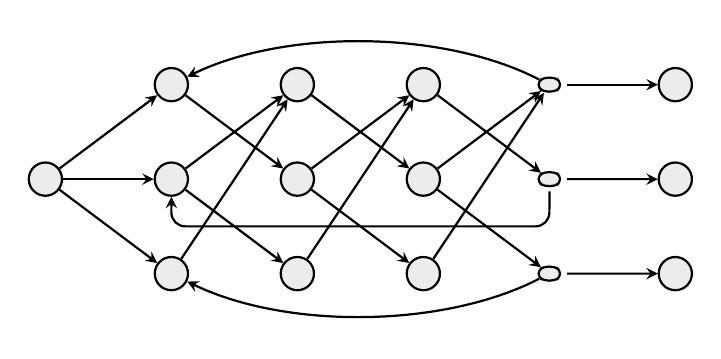
\begin{tikzpicture}[yscale=0.8, xscale=1.6,>=stealth]
\small
		\draw  (0,-1.5)node[player](s){};
  		\path 	(1,0)node[player](a1){}
			++(0,-1.5)node[player](b1){}
			++(0,-1.5)node[player](c1){}
			;
  		\path 	(2,0)node[player](a2){}
			++(0,-1.5)node[player](b2){}
			++(0,-1.5)node[player](c2){}
			;
  		\path 	(3,0)node[player](a3){}
			++(0,-1.5)node[player](b3){}
			++(0,-1.5)node[player](c3){}
			;
		\path 	(4,0)node[random](a4){}
			++(0,-1.5)node[random](b4){}
			++(0,-1.5)node[random](c4){}
			;
		\path 	(5,0)node[player](g1){}
			++(0,-1.5)node[player](g2){}
			++(0,-1.5)node[player](g3){}
			;	
			
		\path [->, thick]
			(s) edge (a1)
			(s) edge (b1)
			(s) edge (c1)
			(a1) edge (b2)
			(a2) edge (b3)
			(a3) edge (b4)
			(b1) edge (c2)
			(b2) edge (c3)
			(b3) edge (c4)
			(c1) edge (a2)
			(c2) edge (a3)
			(c3) edge (a4)
			(b1) edge (a2)
			(b2) edge (a3)
			(b3) edge (a4)
			(a4) edge (g1)
			(b4) edge (g2)
			(c4) edge (g3)
			;
		\draw[->,thick, bend right, out= -45 , in=-135]	(a4) edge (a1);
		\draw[left,thick,->,rounded corners=5pt]  (b4) -- (4,-2.25) -- (1,-2.25) -- (b1);
		\draw[->,thick, bend left,out= 45 , in=135]	(c4) edge (c1);

 \end{tikzpicture}
 \infull{
 \caption{Illustration of Reduction~\ref{red:TriangletoMDPReach}, with . Vertices drawn as cycle are owned by player~1,
vertices drawn as diamond are random vertices.}
 }
 \inshort{
 \caption{Illustration of Reduction~\ref{red:TriangletoMDPReach}, with  . Vertices drawn as cycle are owned by player~1,
vertices drawn as diamond are random vertices.}
 }
 
 \label{fig:TriangletoMDPReach}
\end{figure}
The reduction is illustrated in Figure~\ref{fig:TriangletoMDPReach}.  \infull{
As all random choices are uniformly at random we omit the exact probabilities in the figures.

}
Next we prove that Reduction~\ref{red:TriangletoMDPReach} is indeed a valid reduction 
from triangle detection to disjunctive reachability queries in MDPs.

\begin{lemma}
A graph  has a triangle iff  is contained in , where 
 is the MDP  given by Reduction~\ref{red:TriangletoMDPReach} and   for .
\end{lemma}
\begin{proof}
 For the only if part assume that  has a triangle with vertices  and 
 let ,, be the copies of  in .
 Now a strategy for player~1 in the MDP  to reach  with probability~1 is as follows:
 When in , go to ; when in , go to ; when in , go to ;
 when in , go to .  
 As  form a triangle, all the edges required by the above strategy exist.
 When player~1 starts in  and follows the above strategy the only random vertex he 
 encounters is .
 The random choice sends him to the target vertex  and to vertex 
 with probability  each.
 In the former case he is done, in the latter case he continues playing his strategy and will reach  again after three steps.
 The probability that player~1 has reached  after  steps is 
 which converges to  with  going to infinity.
 Thus we have found a strategy to reach  with probability .

 For the if part assume that . 
 That is, there is an  such that .
 Let us consider a corresponding strategy for reaching .
 First, assume that the strategy would visit a vertex  for . 
 Then with probability  player~1 would end up in the vertex  which has no path to , 
 a contradiction to . 
 Thus the strategy has to avoid visiting vertices  for .
 Second, as the only way to reach  is , the strategy has to choose .
 But then with probability  it will be send to 
 and there must be a path from  to  that doesn't not cross .
 By the latter this path must be of the form  for some .
 Now by the construction of  in the MDP  the vertices  form a triangle in the original graph .
\end{proof}

The size and the construction time of the MDP , constructed by Reduction~\ref{red:TriangletoMDPReach}, is linear in the size of the 
original graph  and we have  target sets.
Thus if we would have a combinatorial  or 
 algorithm for 
disjunctive queries of reachability objectives in MDPs for any , we
would immediately get a combinatorial   algorithm for 
triangle detection, which contradicts STC and BMM.

Next we present a lower bound for sparse MDPs based on OVC and SETH.

\begin{theorem}\label{thm:reach_OVChard}
  There is no  or  algorithm
  \upbr{for any } for 
  disjunctive reachability queries in MDPs under Conjecture~\ref{conj:ov} \upbr{i.e., unless OVC and SETH fail}.
  \infull{In particular, there is no such algorithm deciding whether the winning set is non-empty
  or deciding whether a specific vertex is in the winning set.}
\end{theorem}

To prove the above we give a reduction from OVC to disjunctive reachability queries
in MDPs.

\begin{reduction}\label{red:OVtoMDPReach}
 Given two sets  of -dimensional vectors, we build the following MDP~.  
 \begin{itemize}
  \item The vertices  of the MDP~
  are given by a start vertex~, vertices  and  representing the 
  sets of vectors, vertices  representing the 
  coordinates, and absorbing vertices .
  The edges  of~ are defined as follows: the start vertex~
  has an edge to every vertex of  and every vertex  has an edge to 
  and to its corresponding absorbing vertex ; further for each 
  there is an edge \emph{to}  iff  and for each 
  there is an edge \emph{from}  iff .
	  
  \item The set of vertices  is partitioned into player~1 vertices 
	and random vertices .
	The probabilistic transition function for each vertex  chooses among 's successors
	uniformly at random.
 \end{itemize}
\end{reduction}

\begin{figure}
 \centering
 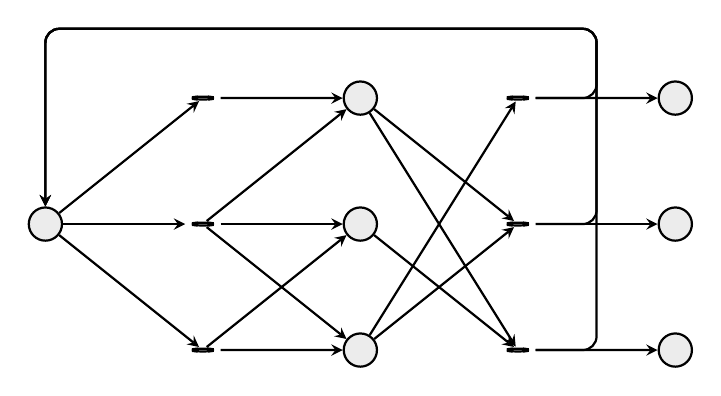
\begin{tikzpicture}[yscale=0.8,>=stealth]
\footnotesize
 \tikzstyle{vrandom}=[draw, thick, diamond, rounded corners, fill=gray!15,inner sep=0.5pt, minimum width=12pt]
  		\path 	node[player](s){}
			++(2,2) node[vrandom](x1){}
			++(0,-2)node[vrandom] (x2){}
			++(0,-2) node[vrandom](x3){}
			(4,2) node[player](c1){}
			++(0,-2) node[player](c2){}
			++(0,-2) node[player](c3){}
			(6,2) node[vrandom](y1){}
			++(0,-2)node[vrandom] (y3){}
			++(0,-2) node[vrandom](y4){}
			(8,2) node[player](g1){}
			++(0,-2)node[player] (g3){}
			++(0,-2) node[player](g4){}
			;
		\normalsize
		\path [->, thick]
			(s) edge (x1)
			(s) edge (x2)
			(s) edge (x3)
			(x1) edge (c1)
			(x2) edge (c1)
			(x2) edge (c2)
			(x2) edge (c3)
			(x3) edge (c2)
			(x3) edge (c3)
			[<-]
			(y1) edge (c3)
			(y3) edge (c1)
			(y3) edge (c3)
			(y4) edge (c1)
			(y4) edge (c2)
			[->]
 			(y1) edge (g1)    
 			(y3) edge (g3)    
 			(y4) edge (g4)  
			;		
		\draw (7,3.1) coordinate[](rc);
		\draw (0,3.1) coordinate[](lc);
		\draw[left,thick,->,rounded corners=5pt]  (y1) -- ++(1,0) -- (rc) -- (lc) -- (s);
		\draw[left,thick,->,rounded corners=5pt]  (y3) -- ++(1,0) -- (rc) -- (lc) -- (s);
		\draw[left,thick,->,rounded corners=5pt]  (y4) -- ++(1,0) -- (rc) -- (lc) -- (s);

 \end{tikzpicture}
  \infull{
 \caption{Illustration of Reduction~\ref{red:OVtoMDPReach} 
	  for  and .}
 }
 \inshort{
 \caption{Illustration of Reduction~\ref{red:OVtoMDPReach} 
	  for   and .}
 }
 \label{fig:OVtoMDPReach}
\end{figure}
The reduction is illustrated on an example in Figure~\ref{fig:OVtoMDPReach}. 

\begin{lemma}
There exist orthogonal vectors ,  iff  where 
 is the MDP  given by Reduction~\ref{red:OVtoMDPReach} and   for .
\end{lemma}
\begin{proof}
 For the only if part assume that there are orthogonal vectors , .
 Now a strategy for player~1 in the MDP  to reach  with probability~1 is as follows:
 When in , go to ; when in some , go to .
 As  and  are orthogonal, each  reachable from  has an edge to , i.e.,
 for  it must be that .
 When player~1 starts in  and follows the above strategy, 
 he reaches  after three steps. There the random choice sends
 him to the target vertex  and back to vertex  with probability  each.
 In the former case he is done, in the latter case
 he continues playing his strategy and will reach  again after three steps.
 The probability that player~1 has reached  after  steps is ,
 which converges to  with  going to infinity.
 Thus we have found a strategy to reach  with probability .

 For the if part assume that . 
 That is, there is an  such that .
 Let us consider a corresponding strategy for reaching .
 First, assume that the strategy would visit a vertex  for .
 Then with probability  the player would end up in the vertex  which has no path to , 
 a contradiction to . 
 Thus the strategy has to avoid visiting vertices .
 Second, as the only way to reach  is , the strategy has to choose .
 But then with probability  it will be send to 
 and thus there must be a strategy to reach  from  with probability  that does not cross .
 As  is the only predecessor of , there must also be such a strategy to reach .
 In other words, there must be an  such that for each successor  there 
 is an edge to . 
 By the construction of the MDP~ this is equivalent to the existence of
 an   such that whenever  then , 
 and thus  and  are orthogonal vectors.
\end{proof}

The number of vertices in , constructed by Reduction~\ref{red:OVtoMDPReach},
is  and the construction can be performed in 
 time (recall that ). 
The number of edges~ is  (thus we consider 
to be a sparse MDP) and the number of target sets .
Finally, if we would have an   or  algorithm for disjunctive reachability queries in MDPs for any , we
would immediately get an  algorithm for OV, which contradicts OVC (and thus SETH).

\infull{\section{Safety Objectives}\label{sec:safety}
It is well-known that computing the a.s.\ winning set for a single safety objective 
in an MDP is equivalent to computing
the winning set of player~1 for safety objectives in the 2-player graph-game where all the random vertices are owned by the opponent, called player~2 
(see e.g.~\cite{ChatterjeeDH10}).
A 2-player graph-game is defined as a graph with a partition 
of the vertices into player~1 vertices~ and player~2 vertices~. 
A player~2 strategy is defined analogous to a player~1 strategy (replacing the 
vertices~ with the vertices~ in the definition). 
The objective of player~2 is the dual of the objective of player~1.

Safety objectives in 2-player graph-games can be computed in ~time by computing
a player~2 attractor (the definition of a player~1 or player~2 attractor is 
analogous to the definition of a random attractor in Definition~\ref{def:attr}).
Thus in MDPs the a.s.\ winning set for a single safety objective can be computed in ~time by computing a random attractor,
and the a.s.\ winning set for a disjunctive query can be determined 
in  time by computing  random attractors and union the winning sets.
Conjunctive safety can be reduced to a single safety objective in  time 
by taking the union of all the sets .

Turning to disjunctive safety objectives, we have the same equivalence to 2-player graph-games as for single objectives (Observation~\ref{obs:SafetyGames}).
In this 2-player game the disjunctive safety objective is the 
complementary objective to the 
conjunctive reachability objective with the same sets and, as the game is determined~\cite{FijalkowH12}\footnote{A graph-game is determined if the winning 
set of player~1 is the complement of the winning set of player~2.},
the -hardness shown in~\cite{FijalkowH12} also applies to disjunctive safety objectives.

\begin{observation}\label{obs:SafetyGames}
    Computing the a.s.\ winning set for a disjunctive safety objective in an MDP 
    with player~1 vertices~ and random vertices~ is equivalent to 
    computing the same disjunctive safety objective in the 2-player graph-game
    with the same edges and the same player~1 vertices and 
    player~2 vertices~.
\end{observation}
\begin{proof}
 We show that a vertex  is almost sure winning in the MDP if and only if it is winning for player~1 in the game graph.
 
 \noindent  Assume  is not winning for player~1 in the graph-game. 
	       Then  is winning for player~2 and thus player~2 has a strategy to visit all target sets from .
	       As there are only finitely many target sets, all these target sets are visited after a finite number of steps,
	       lets say after  steps.
	       Now consider the corresponding MDP; with some constant probability the random choices in the MDP will follow exactly the strategy of player~2 in the 
	       graph-game for the first 
	       steps and in that case player~1 cannot win almost surely from .
	       Hence,  is not in the a.s.\ winning set.
 
 \noindent  Assume player~1 has a winning strategy for the graph-game
 starting in .
    By definition this strategy is also winning for the MDP (if it is winning for each possible choice of player~2 then it also
    winning for a random choice).
\end{proof}

\subsection{Conditional Lower Bounds for Safety Objectives}\label{subsec:safety_lowerbounds}
}
\inshort{
\subsection{Safety Objectives}\label{subsec:safety_lowerbounds}
}

We first present a lower bound for disjunctive safety based on STC that even holds on graphs.

\begin{theorem}\label{thm:safety_STChard}
  There is no combinatorial  or  algorithm \upbr{for any } for disjunctive safety \upbr{objectives or queries} in graphs under  Conjecture~\ref{conj:triangle} \upbr{i.e., unless STC and BMM fail}. 
  \infull{In particular, there is no such algorithm deciding whether the winning set is non-empty
  or deciding whether a specific vertex is in the winning set.}
\end{theorem}

The above is by the linear time reduction from triangle detection to disjunctive safety in graphs 
provided below.

\begin{reduction}\label{red:TriangletoGraphs}
 Given a graph  \upbr{for triangle detection}, we build a graph  \upbr{for disjunctive safety} as follows.
 As vertices  we have four copies  of  and a vertex .
 A vertex  has an edge to a vertex  iff . 	  
 Finally,  has an edge to all vertices in  and all vertices in  have an edge to~.
\end{reduction}
\begin{figure}
 \centering
 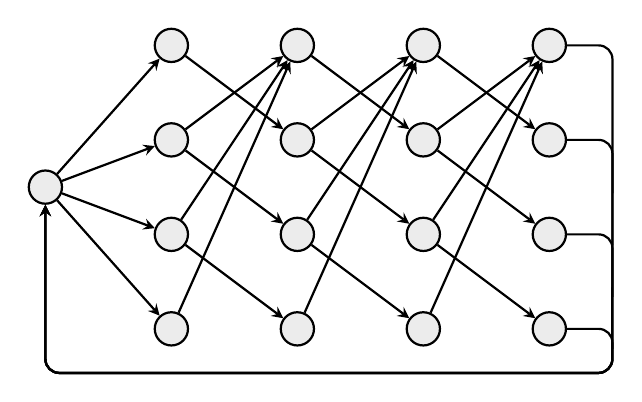
\begin{tikzpicture}[yscale=0.8, xscale=1.6,>=stealth]
\small
		\draw  (0,-2.25)node[player](s){};
  		\path 	(1,0)node[player](a1){}
			++(0,-1.5)node[player](b1){}
			++(0,-1.5)node[player](c1){}
			++(0,-1.5)node[player](d1){}
			;
  		\path 	(2,0)node[player](a2){}
			++(0,-1.5)node[player](b2){}
			++(0,-1.5)node[player](c2){}
			++(0,-1.5)node[player](d2){}
			;
  		\path 	(3,0)node[player](a3){}
			++(0,-1.5)node[player](b3){}
			++(0,-1.5)node[player](c3){}
			++(0,-1.5)node[player](d3){}
			;
		\path 	(4,0)node[player](a4){}
			++(0,-1.5)node[player](b4){}
			++(0,-1.5)node[player](c4){}
			++(0,-1.5)node[player](d4){}
			;
		\path [->, thick]
			(s) edge (a1)
			(s) edge (b1)
			(s) edge (c1)
			(s) edge (d1)
			(a1) edge (b2)
			(a2) edge (b3)
			(a3) edge (b4)
			(b1) edge (c2)
			(b2) edge (c3)
			(b3) edge (c4)
			(c1) edge (a2)
			(c2) edge (a3)
			(c3) edge (a4)
			(b1) edge (a2)
			(b2) edge (a3)
			(b3) edge (a4)
			
			(c1) edge (d2)
			(c2) edge (d3)
			(c3) edge (d4)
			
			(d1) edge (a2)
			(d2) edge (a3)
			(d3) edge (a4)
			;
		\draw[left,thick,->,rounded corners=5pt]  
		(a4) -- ++(0.5,0) -- (4.5,-5.2) -- (0,-5.2) -- (s);
		\draw[left,thick,->,rounded corners=5pt]  
		(b4) -- ++(0.5,0) -- (4.5,-5.2) -- (0,-5.2) -- (s);
		\draw[left,thick,->,rounded corners=5pt]  
		(c4) -- ++(0.5,0) -- (4.5,-5.2) -- (0,-5.2) -- (s);
		\draw[left,thick,->,rounded corners=5pt]  
		(d4) -- ++(0.5,0) -- (4.5,-5.2) -- (0,-5.2) -- (s);


 \end{tikzpicture}
 \infull{
 \caption{Illustration of Reduction~\ref{red:TriangletoGraphs}, with  .
 The target sets for disjunctive safety are , , , and .
 }
 }
 \inshort{
 \caption{Illustration of Reduction~\ref{red:TriangletoGraphs}, with  .
 The target sets for disjunctive safety are , , , and .}
 }
 \label{fig:TriangletoGraphs}
\end{figure}
Reduction~\ref{red:TriangletoGraphs} is illustrated in Figure~\ref{fig:TriangletoGraphs}.

\begin{lemma}
 Let  be the graph given by Reduction~\ref{red:TriangletoGraphs} for a graph~
 and  
 let . Then 
    \infull{the following statements are equivalent.
  \begin{enumerate}
  \item
   has a triangle.
  \item  is in the winning set of  .
  \item The winning set of  is non-empty.
  \end{enumerate}
  }
  \inshort{ has a triangle iff  is in the winning set of  .}
\end{lemma}
\begin{proof}
 \infull{(1)(2): Assume}\inshort{For the only if part assume} that
  has a triangle with vertices  and 
 let ,, be the copies of  in .
 Now a strategy for player~1 in  to satisfy  is as follows:
 When in , go to ; when in , go to ; when in , go to ;
 when in , go to ; and when in , go to .
 As  form a triangle, all the edges required by the above strategy exist.
 When player~1 starts in~ and follows the above strategy,
 then he plays an infinite path
 that only uses vertices  and thus satisfies .

 \infull{(2)(1): Assume}\inshort{For the if part assume} that there is a
 winning play starting in  and satisfying .
 Starting from , this play has to first go to , as all other successors of  would violate
 the safety constraint. Then the play continues on some vertex  and 
 and then, again by the safety constraint, has to enter .
 Now by construction of  we know that there must be edges  in the original graph ,
 i.e.\ there is a triangle in .  \infull{
 
 (2)(3): Notice that when removing  from  we get an acyclic graph and thus each infinite
 path has to contain  infinitely often. Thus, if the winning set is non-empty,
 there is a cycle winning for some vertex and then 
 this cycle is also winning for . For the converse direction we have that if  is in the winning set, then the winning set is non-empty.}
\end{proof}

The size and the construction time of the graph , constructed 
by Reduction~\ref{red:TriangletoGraphs}, is linear in the size of the 
original graph  and we have  target sets.
Thus if we would have a combinatorial   or  algorithm for disjunctive 
safety objectives or queries in graphs, we
would immediately get a combinatorial   algorithm for triangle detection, which contradicts STC (and thus BMM).

The above reduction uses a linear number of safety constraints which are all of linear size. 
Thus, a natural question is whether smaller safety sets would make the problem any easier. 
Next we argue that our result even holds for safety sets that are of logarithmic size.
To this end we modify Reduction~\ref{red:TriangletoGraphs} as follows. We remove all edges incident to  and 
replace them by two complete binary trees. The first tree with  as root and the vertices  as leaves is directed towards the leaves, 
the second tree with root~ and leaves~ is directed towards~.
Now for each pair  one can select one vertex of each level of the trees (except for the root levels) 
for the set  such that the only safe path starting in  has to use 
 and each safe path to  must pass .
As the depth of the trees is logarithmic in the number of leaf vertices, we get
sets of logarithmic size. 
The construction with the binary trees 
is illustrated in Figure~\ref{fig:TriangletoGraphs_tree}.
\begin{figure}
\centering
 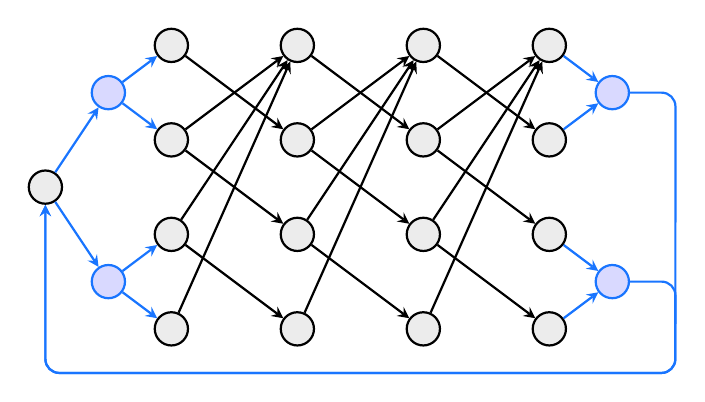
\begin{tikzpicture}[yscale=0.8, xscale=1.6,>=stealth]
\tikzstyle{trcolor}=[color=blue!60!cyan!90!white,text=blue!60!cyan!80!black]
\tikzstyle{playerc}=[player,trcolor,fill=blue!15,]
\tikzstyle{edgec}=[thick,trcolor]
 \small
		\draw  (0,-2.25)node[player](s){};
		\path (0.5,-0.75)node[playerc](x1){}
			++(0,-3)node[playerc](x2){}
			;
  		\path 	(1,0)node[player](a1){}
			++(0,-1.5)node[player](b1){}
			++(0,-1.5)node[player](c1){}
			++(0,-1.5)node[player](d1){}
			;
  		\path 	(2,0)node[player](a2){}
			++(0,-1.5)node[player](b2){}
			++(0,-1.5)node[player](c2){}
			++(0,-1.5)node[player](d2){}
			;
  		\path 	(3,0)node[player](a3){}
			++(0,-1.5)node[player](b3){}
			++(0,-1.5)node[player](c3){}
			++(0,-1.5)node[player](d3){}
			;
		\path 	(4,0)node[player](a4){}
			++(0,-1.5)node[player](b4){}
			++(0,-1.5)node[player](c4){}
			++(0,-1.5)node[player](d4){}
			;
		\path (4.5,-0.75)node[playerc](y1){}
			++(0,-3)node[playerc](y2){}
			;
		\path [->, thick]			
			(a1) edge (b2)
			(a2) edge (b3)
			(a3) edge (b4)
			(b1) edge (c2)
			(b2) edge (c3)
			(b3) edge (c4)
			(c1) edge (a2)
			(c2) edge (a3)
			(c3) edge (a4)
			(b1) edge (a2)
			(b2) edge (a3)
			(b3) edge (a4)
			
			(c1) edge (d2)
			(c2) edge (d3)
			(c3) edge (d4)
			
			(d1) edge (a2)
			(d2) edge (a3)
			(d3) edge (a4)
			;
		\path [->,edgec]
			(s) edge (x1)
			(s) edge (x2)
			(x1) edge (a1)
			(x1) edge (b1)
			(x2) edge (c1)
			(x2) edge (d1)
			(a4) edge (y1)
			(b4) edge (y1)
			(c4) edge (y2)
			(d4) edge (y2)
			;
		\draw[left,edgec,->,rounded corners=5pt]  
		(y1) -- ++(0.5,0) -- (5,-5.2) -- (0,-5.2) -- (s);
		\draw[left,edgec,->,rounded corners=5pt]  
		(y2) -- ++(0.5,0) -- (5,-5.2) -- (0,-5.2) -- (s);

 \end{tikzpicture}
  \caption{Illustration of how to reduce the number of entries in the target sets in Reduction~\ref{red:TriangletoGraphs} with two complete binary trees. Here
   and the target sets
  for disjunctive safety are , 
  , , and 
  .}
 \label{fig:TriangletoGraphs_tree}
\end{figure}

Next we present an  lower bound for disjunctive objective/query safety in sparse MDPs.

\begin{theorem}\label{thm:safety_OVChard}
  There is no  or  algorithm \upbr{for any } for disjunctive safety objectives/queries in MDPs under Conjecture~\ref{conj:ov} \upbr{i.e., unless
  OVC\infull{ and }\inshort{ \& }SETH fail}.
  \infull{In particular, there is no such algorithm for deciding whether the winning set is non-empty
  or deciding whether a specific vertex is in the winning set.}
\end{theorem}

To prove the above, we give a linear time reduction from OV to disjunctive safety objectives/queries.

\begin{reduction}\label{red:OVtoMDPsafety}
 Given two sets  of -dimensional vectors, we build the following MDP~.  
 \begin{itemize}
  \item   The vertices  of the MDP~
  are given by a start vertex~, vertices  and  representing the 
  sets of vectors, and 
  vertices  representing the 
  coordinates. The edges  of~ are defined as follows: the start vertex~
  has an edge to every vertex of  and every vertex  has an edge to ;
  further for each 
  there is an edge \emph{to}  iff  and for each 
  there is an edge \emph{from}  iff .
  \item The set of vertices  is partitioned into player~1 vertices 
	and random vertices .
	Moreover, the probabilistic transition function for each vertex  chooses among 's successors
	uniformly at random.	
 \end{itemize}
\end{reduction}
The reduction is illustrated on an example in Figure~\ref{fig:OVtoMDPsafety}. 

\begin{lemma}\label{lem:OVtoMDPsafety}
  Given two sets  of -dimensional vectors,
  the corresponding MDP  given by Reduction~\ref{red:OVtoMDPsafety} and  
   for 
  the following statements are equivalent
  \begin{enumerate}
    \item There exist orthogonal vectors , .
    \item 
    \item 
    \infull{\item The winning set  is non-empty.
    \item The winning set  is non-empty.}
  \end{enumerate}
\end{lemma}
\begin{proof}
 W.l.o.g.\ we assume that the -vector, i.e., the vector with all coordinates being , is  contained in 
 (adding the -vector does not change the result of the OV instance).
 Then a play in the MDP  proceeds as follows. 
 Starting from , player~1 chooses a vertex ; then a vertex
 
 and then a vertex  are picked randomly; then the play goes 
 back to , starting another cycle of the play.
 
 (1)(2): Assume there are orthogonal vectors , .
    Now player~1 can satisfy  in the MDP  
    by simply going to  whenever the play is in .
    The random player will then send it to some adjacent 
    and then to some adjacent vertex in , 
    but as  and  are orthogonal, this  is not connected to . 
    Thus the play will never visit .
 
 (2)(3): Assume . Then 
    there is a vertex  such that . 
    Now we can enlarge the objective
    to  and obtain
    .
 
 (3)(1): Assume  and consider
    a corresponding strategy~. 
    W.l.o.g.\ we can assume that this strategy is memoryless~\cite{Thomas95}. 
    Thus whenever the play is in~, it picks a fixed  as the next vertex.
    Assume towards contradiction that there is no orthogonal vector   for .
    Then for each  we have that there is a  connecting  to .
    In each cycle of the play one goes from  to  and then by random choice to some vertex in .
    By the above, each of the vertices in  has a non-zero probability to be 
    reached in this cycle, which can, for each fixed ,
    be lower bounded by a constant .
    Thus after  cycles in the play with probability at least  
    all vertices in  have been visited and thus none of the safety objectives is 
    satisfied, a contradiction to the assumption that with probability~ at least one
    safety objective is satisfied.
    Thus there must exist a vector  orthogonal to~.\infull{
  
  (2)(4) \& (3)(5): 
     Notice that when removing  from  we get an acyclic MDP and 
     thus each infinite
     path has to contain  infinitely often. 
     Certainly if  is in the a.s.\ winning set, this set is non-empty. 
     Thus let us assume there is a vertex  different from  with a winning strategy .
     All (winning) paths starting in  cross  after at most  steps and thus 
      must be also winning when starting in .}
\end{proof}
  \begin{figure}
  \centering
  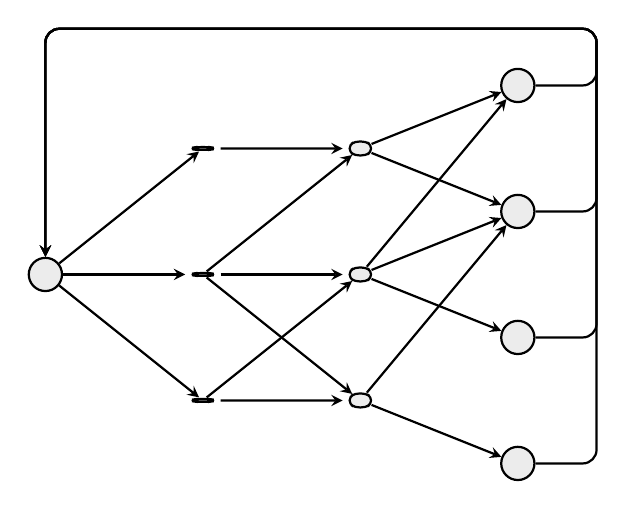
\begin{tikzpicture}[yscale=0.8,>=stealth]
\footnotesize
  		\path 	node[player](s){}
			++(2,2) node[vrandom](x1){}
			++(0,-2)node[vrandom] (x2){}
			++(0,-2) node[vrandom](x3){}
			(4,2) node[random](c1){}
			++(0,-2) node[random](c2){}
			++(0,-2) node[random](c3){}
			(6,3) node[vplayer](y1){}
			++(0,-2) node[vplayer](y2){}
			++(0,-2)node[vplayer] (y3){}
			++(0,-2) node[vplayer](y4){}
			;
		\normalsize
		\path [->, thick]
			(s) edge (x1)
			(s) edge (x2)
			(s) edge (x3)
			(x1) edge (c1)
			(x2) edge (c1)
			(x2) edge (c2)
			(x2) edge (c3)
			(x3) edge (c2)
			(x3) edge (c3)
			[<-]
			(y1) edge (c1)
			(y1) edge (c2)
			(y2) edge (c1)
			(y2) edge (c2)
			(y2) edge (c3)
			(y3) edge (c2)
			(y4) edge (c3)
			;
			
		\draw[left,thick,->,rounded corners=5pt]  (y1) -- ++(1,0) -- (7,3.9) -- (0,3.9) -- (s);
		\draw[left,thick,->,rounded corners=5pt]  (y2) -- ++(1,0) -- (7,3.9) -- (0,3.9) -- (s);
		\draw[left,thick,->,rounded corners=5pt]  (y3) -- ++(1,0) -- (7,3.9) -- (0,3.9) -- (s);
		\draw[left,thick,->,rounded corners=5pt]  (y4) -- ++(1,0) -- (7,3.9) -- (0,3.9) -- (s);

  \end{tikzpicture} 
   \infull{
      \caption{Illustration of Reduction~\ref{red:OVtoMDPsafety}, for  and 
    .}
   }
   \inshort{
      \caption{Illustration of Reduction~\ref{red:OVtoMDPsafety}, for   and 
     .}
   }
  \label{fig:OVtoMDPsafety}
  \end{figure}

The number of vertices in the MDP~, constructed by Reduction~\ref{red:OVtoMDPsafety}, is , the number of edges~ is  
(recall that ), we have  target sets, and the construction can be performed in 
 time.
Thus, if we would have an  or 
algorithm for disjunctive 
queries or disjunctive objectives of safety objectives for any , we
would immediately get an   algorithm for OV, which contradicts OVC (and thus SETH).

\section{Algorithms for MDPs with Streett objectives}\label{sec:streett}

In this section we extend algorithms for graphs with Streett objectives to MDPs. 
In particular we prove the following theorem.
\begin{theorem}
	For an MDP~ with Streett objectives defined by Streett pairs 
	 with 
	
	the almost-sure winning set can be computed in  time.\footnote{It can also be computed in 
	 time, which is faster for some combinations
	of parameters with .}
\end{theorem}

We first describe the basic algorithm for MDPs with Streett objectives, which 
uses an algorithm for MEC-decomposition as a black box. We then develop a new 
algorithm that opens up this black box and after an initial computation of the 
MEC-decomposition only uses strongly connected components
and random attractor computations\infull{ (Section~\ref{sec:streettimpr})}. 
This algorithm reveals strong similarities to the known algorithms for graphs 
with Streett objectives. We then extend the two approaches that lead to the best
asymptotic running times on graphs, one for dense 
graphs\infull{ (Section~\ref{sec:streettdense})} 
and one for sparse\infull{ (Section~\ref{sec:streettdense})}
graphs, to MDPs. The algorithms for graphs are based on finding
``good'' strongly connected subgraphs and then determining which vertices can
reach these ``good components''. For MDPs we find \emph{good end-components}
and then compute almost-sure reachability with the union of all good 
end-components as target set
to determine the almost-sure winning set.
We first show that this approach is correct\infull{ 
(Section~\ref{sec:gec}, see also~\cite[Chap.~10.6.3]{baierbook})}
and then provide algorithms that identify all good end-components.

\subsection{Good End-Components}\label{sec:gec}

Good end-components are also useful for other objectives such as Rabin objectives.
The results of this subsection are valid for all objectives for which whether
an infinite path  belongs to the objective depends only on the vertices
 that occur infinitely often in .
For such objectives we show that determining the winning set is equivalent to 
computing almost-sure reachability of the union of all good end-components.
We define a good end-component as an end-component for which the objective
is satisfied if exactly the vertices of the end-component are visited infinitely
often.
\begin{definition}[Good End-Component]\label{def:good_ec}
  Given an MDP  and an objective ,
  an end-component  of  such that
  each path  with  is in 
  is called a \emph{good ~end-component}.
\end{definition}
For a Streett objective the following is an equivalent definition.
\begin{definition}[Good Streett End-Component]
	Given an MDP  and a set  of
	Streett pairs, 
	a \emph{good Streett end-component} is an end-component  of  such that
	for each  either  or
	.
\end{definition}

The importance of end-components lies in the fact that player~1 can keep the play
in an end-component forever and can visit each vertex in the end-component
almost surely and also almost surely infinitely often
(Lemma~\ref{lem:ec_vist_infinitly}). This implies that in a good end-component
player~1 has an almost-sure winning strategy (Lemma~\ref{lem:wingood}) and thus
player~1 has an almost-sure winning strategy from every vertex that can 
almost-surely reach a good end-component (Lemma~\ref{lem:reachwin} and 
Corollary~\ref{cor:gecsound-gen}). This shows the soundness of the approach
of determining the almost-sure winning set for an objective determined by 
 by computing almost-sure reachability of the union of all good
end-components.

\begin{lemma}\label{lem:ec_vist_infinitly}
  Given an MDP  and an end-component~, player~1 has a strategy
  from each vertex of  such that all vertices of~ are 
  almost-surely reached infinitely often
  and only vertices of~ are visited. 
\end{lemma}
\begin{proof}
  We define a strategy  as follows: 
  Choose some arbitrary numbering of the vertices in~. The (not memoryless)
  strategy of player~1 is to first follow a shortest path within the end-component
  (with, say, lexicographic tie breaking) to the first vertex from the current 
  position of the play until this vertex is reached, then a shortest path 
  within the end-component to the 
  second vertex and so on, until he starts with the first vertex again. This is
  possible because an end-component is a strongly connected subgraph. 
  Since an end-component has no outgoing random edges, the 
  play does not leave the end-component when player~1 plays this strategy.
  Let  and let  be the smallest
  positive transition probability in the MDP. Then the probability that the first 
  chosen shortest path is followed with the above strategy 
  is at least  and the 
  probability that a sequence of  shortest paths within  are followed 
  and thus all vertices of  are visited is at least . Thus 
  the probability that not all 
  vertices in  were visited after  steps is at most , which goes to 0 when  goes to infinity. Hence player~1
  has a strategy such that all vertices in  are visited with probability~1.
  By the same argument all vertices in  are visited infinitely often with 
  probability~1 because the probability that some vertex is not visited after 
  some finite prefix of length  can be bounded by .
\end{proof}

\begin{lemma}\label{lem:wingood}
  Player~1 has a strategy  from each vertex in a good  end-component~
  to satisfy  almost-surely.
\end{lemma}
\begin{proof}
  By Lemma~\ref{lem:ec_vist_infinitly} player~1 has a strategy that almost-surely visits
  all nodes in  infinitely often. By the definition of good  end-component, 
  all paths visiting all nodes in  infinitely often are in .
  Hence, the strategy given by Lemma~\ref{lem:ec_vist_infinitly} is also almost-sure winning for~.
\end{proof}

\begin{lemma}\label{lem:reachwin}
  Given an MDP , an objective  that is determined by ,
  and a set  of almost-sure winning nodes we have that 
  if , then also .
\end{lemma}
\begin{proof}
 Assume  and consider the following strategy.
 Start with the strategy for reaching  and as soon as one vertex  of  is reached 
 switch to the almost-sure winning strategy of .
 As  is (almost-surely) reached within a finite number of steps, the vertices
 visited by the strategy for reaching  does not affect the objective .
\end{proof}

\begin{corollary}[Soundness of Good End-Components]\label{cor:gecsound-gen}
  For a set of good end-components~ and an objective  that is determined by 
  we have that   is contained in .
\end{corollary}

Another conclusion we can draw from the above lemmata is that if a MEC contains
a good end-component, then player~1 has an almost-sure winning strategy
for the whole MEC because he can reach the good end-component almost-surely from 
every vertex of the MEC. We exploit this observation in the improved algorithm 
for coBüchi objectives in Section~\ref{sec:cobuchialg}.
\begin{corollary}[of Lemmata~\ref{lem:ec_vist_infinitly} 
and~\ref{lem:reachwin}]\label{cor:winning_mec}
  Given an MDP  and an objective  that is determined by ,
  if a MEC  contains an almost-sure
  winning vertex \upbr{e.g.\ a good end-component~},
  then all vertices in  are almost-sure winning for player~1.
\end{corollary}

To show the completeness of the approach of computing good end-components,
we have to argue that every vertex from which player~1 can satisfy the objective 
almost-surely has also a strategy to reach a good end-component almost-surely.
For this we need two rather technical lemmata.
The intuition behind Lemma~\ref{lem:zeroprob_paths} is that if a random vertex 
occurs infinitely often on a path,
then almost-surely also each of its successors appears infinitely often on that 
path. Thus we can argue that vertex sets that are reached infinitely often 
with positive probability are closed under random edges and hence SCCs within such 
sets of vertices are end-components (Lemma~\ref{lem:random_closure}). 
To show completeness (Proposition~\ref{prop:geccompl-gen})
we then use a set of paths in the objective that are reached with positive 
probability to show that the vertices that these paths use infinitely often 
form good end-components. A similar proof is given for Büchi objectives in
\cite{CourcoubetisY95}. 

\begin{lemma}\label{lem:zeroprob_paths}
  Given an MDP , a strategy  of player~1,
  the set  of infinite paths starting at a vertex  that are compatible with the strategy , and
  a vertex  with ,
  for each successor  of  we have  
    and
  .
\end{lemma}
\begin{proof}
  Whenever the strategy visits node , with some constant probability  the play continues in .
  Thus the probability that  was visited less than  times after  was visited  times
  is upper bounded by  which goes to  with increasing .
  Thus, we have 
  and hence for the complement set .
\end{proof}

\begin{lemma}\label{lem:random_closure} 
  Given an MDP , a strategy  of player~1,
  the set  of infinite paths starting at a vertex  that are compatible with the strategy , 
  a set , and the set of vertices 
  , then
  for each SCC  of  and each vertex  all successors of a are contained in , i.e.,  is an end-component of .
\end{lemma}
\begin{proof}
 Consider an SCC , a vertex , and a successor .
 Then by definition  
 for a  and by Lemma~\ref{lem:zeroprob_paths} 
 we get  
 and thus  ,
 i.e., .
 For each of the paths  in the latter set we have a path from  to  consisting solely of nodes in .
 As in  there are just finitely many paths from  to  at least one must have non-zero probability 
 and thus is also contained in .  Hence,  belongs to the SCC .
\end{proof}

\begin{proposition}[Completeness of Good End-Components]\label{prop:geccompl-gen}
    Given an MDP  with an objective  determined by 
    and let  be the set of all good  end-components,
    then  is contained in  .
\end{proposition}
\begin{proof}
  For a vertex ,
  fix a strategy  of player~1 such that the objective is satisfied almost-surely. 
  Let  be the sub-MDP of  that consists of the vertices that 
  are visited infinitely often with non-zero probability when player~1 follows strategy~.
  Note that by Lemma~\ref{lem:random_closure} each SCC of  is an 
  end-component of .
  Moreover,  is a strategy for almost-surely reaching  
  (each infinite path has to visit at least one vertex infinitely often).
  
  It remains to show that each vertex of  can almost-surely reach 
  a good end component. 
  We will actually show that each vertex of  is already contained in a good end component.
  To this end let  be the set of infinite paths starting at~
  that are compatible with the strategy  and satisfy the objective.
  For an arbitrary node  of  we consider all paths 
   with  and group them by .
  At least one of these groups has non-zero probability, 
  as there are only finitely many possible sets  and  has non-zero probability.  
  Let us consider one of the groups of paths  with non-zero probability 
  and the corresponding set  for .
  By Lemma~\ref{lem:random_closure} the set  is closed under random edges.
  Moreover, as in each path  the vertices  are strongly connected, the
  set  is also strongly connected and thus an end-component.
  Finally, as the paths  satisfy the objective
  and the objective  is determined by , the set 
  forms a good end component.
  Hence, we have shown that each vertex of  is contained in a good  
  end-component, which completes the proof.
\end{proof}

\subsection{Algorithm Preliminaries}\label{sec:algprelim}
We introduce some additional notation for the algorithms for MDPs with Streett 
and Rabin objectives.
For a set 
of Rabin pairs or a set , 
let .
A \emph{strongly connected component} \upbr{SCC} is a \emph{maximal} strongly 
connected subgraph. A single vertex is considered strongly connected. An SCC without
outgoing edges is a \emph{bottom SCC}, one without incoming edges a \emph{top SCC}.
The \emph{reverse graph}  is constructed by reversing the direction of 
all edges of the graph . In a graph  the set of vertices  
for some vertex  denotes the set of vertices  for which .
The out-degree of  in  is denoted with , its in-degree
with . Let \textsc{MEC} denote the runtime to compute the maximal 
end-component decomposition of an MDP; we assume .
Further we assume that each vertex in the input MDP 
has at least one outgoing edge, and thus we have .

\begin{definition}[Random Attractor]\label{def:attr}
In an MDP  
the \emph{random attractor}  of a set of vertices 
 is defined as  where  and 
 for  is defined recursively as .
The random attractor  can be computed in  time~\cite{Beeri80,Immerman81}.
\end{definition}

All the algorithms for Streett objectives maintain vertex sets that are 
candidates for good end-components. For such a vertex set~ we (a) 
refine the maintained sets according to the SCC decomposition of 
and (b) for a set of vertices~ for which we know that it cannot be contained 
in a good end-component, we remove its random attractor from . The following lemma 
shows the correctness of these operations.

\begin{lemma}\label{lem:eccontained}
	Given an MDP , let  be an end-component with  for 
	some . 
	We have 
	
	\begin{itemize}
	 \item[\upbr{a}] for one SCC~ of  and
	 
	 \item[\upbr{b}]  for each 
			 and each sub-MDP~ containing~.
	\end{itemize}
\end{lemma}

\begin{proof}
	Property \upbr{a} holds since every end-component induces a strongly connected
	sub-MDP. We prove Property \upbr{b} by showing that 
	does not contain a vertex of  by induction over the recursive 
	definition of a random attractor. Let the sets  be as in
	Definition~\ref{def:attr} and let  be the vertices to which  has an 
	edge in~. 
	We have  and thus .
	Assume we have  for some . No vertex of
	 has an outgoing edge to  and thus the set 
	 is empty.
	Further every vertex in  has an outgoing edge to a vertex in .
	Hence also  is empty
	and we have that .
\end{proof}

Let  be a good Streett end-component. Then  implies 
. Thus if  for some vertex 
set  and some index , then we have  
for each end-component~. Hence we obtain the 
following corollary.

\begin{corollary}\label{cor:geccontained}
Given an MDP , let  be a \emph{good} Streett end-component with 
 for some . 
For each  with  it holds that 
.
\end{corollary}

\subsection{Improving Upon the Basic Algorithm}\label{sec:streettimpr}

In Algorithm~\ref{alg:streettbasic}, the basic algorithm for MDPs with Streett 
objectives, we maintain a set of already identified 
(maximal) good end-components~, which is initially empty, and a set of 
candidate end-components~, which is initialized with the 
MECs of the input MDP~. In each iteration of the while-loop we remove 
an end-component  from  and check whether it is a 
good end-component. For this check we find sets  for  
that do not intersect with  and identify vertices in  for 
such an  as ``bad vertices''~. If there are no bad vertices, then
 is a good end-component and added to . Otherwise the bad 
vertices and their random attractor within  are removed from .
On the sub-MDP induced by the remaining vertices of  we compute the 
MEC-decomposition, which identifies all remaining candidate end-components among
the vertices of . The new candidates are then added to .
If the algorithm finds good end-components, it returns the almost-sure winning set
for the reachability of the union of them.

\begin{algorithm}
	\SetAlgoRefName{StreettMDPbasic}
	\caption{Basic Algorithm for MDPs with Streett Objectives}
	\label{alg:streettbasic}
	\SetKwInOut{Input}{Input}
	\SetKwInOut{Output}{Output}
	\BlankLine
	\Input{an MDP  and Streett pairs 
	
	}
	\Output
	{
	
	}
	\BlankLine
	\;
	\;
	\While{}{
		remove some  from \;
		\;
		\If{}{
			\label{lbasic:remove}\;
			\label{lbasic:mec}\;
		}\Else{
			\;
		}
	}
	\Return{}\;
\end{algorithm}

\begin{proposition}[Runtime of 
Algorithm~\ref{alg:streettbasic}]\label{prop:timestreetbasic}
	Algorithm~\ref{alg:streettbasic} can be implemented 
	to run in  time.
\end{proposition}

\begin{proof}
	The initialization of  with all MECs of the input
	MDP  can clearly be done in  time. Further by 
	Theorem~\ref{th:timedrmdp} the almost-sure reachability computation
	after the while-loop can be done in  time. 
	
	Let  denote the end-component of  currently containing 
	an arbitrary, fixed vertex  during Algorithm~\ref{alg:streettbasic}. 
	In each iteration
	of the while-loop in which  is considered either (a) 
	and  will not be considered further or (b) the number of vertices
	in  is reduced by at least one and we have for some  that
	 before the iteration of the while-loop and
	 after the while-loop. Thus each vertex and 
	each edge of the MDP  is considered in at most  iterations
	of the while-loop.
	
	Consider the th iteration of the while-loop; let  denote the set 
	removed from  in this iteration and let . 
	Assume that each vertex has a list of the sets  and  for 
	 it belongs to.
	(We can generate these lists from the lists of the Streett pairs in 
	time at the beginning of the algorithm.)
	Then we can determine  by going through all lists of the vertices 
	in  in  time, which amounts to 
	 total time over all iterations of the while-loop.
	The random attractor computed in Line~\ref{lbasic:remove} is removed and 
	not considered further, thus its computation takes  time over the whole 
	algorithm (see Definition~\ref{def:attr}). The computation
	of all MECs in  takes total time 
	over all iterations of the while loop. Thus the whole algorithm can be 
	implemented in  total time.
\end{proof}

\begin{proposition}[Soundness of Algorithm~\ref{alg:streettbasic}]
	Let  be the set returned by Algorithm~\ref{alg:streettbasic}.
	We have .
\end{proposition}

\begin{proof}
By Corollary~\ref{cor:gecsound-gen} it is sufficient to show that every set 
 is a good end-component. The algorithm explicitly
checks immediately before  is added to  that we have for each 
 either  or . Thus it only remains
to show that  is an end-component when it is added to . Before 
a set is added to , the same set is contained in the set . 
We show that all sets in  are end-components at any point in 
the algorithm by induction over the iterations of the while-loop in the algorithm. 
Before the first iteration of the while-loop the sets  are
the maximal end-components of . Now consider an iteration in which
a set  is removed from  and new sets are added to 
. First, some vertices and their random attractor in the 
sub-MDP  induced by  are removed from . Let  be the 
remaining set of vertices. By the definition of a random attractor there are no 
random edges from  to the removed random attractor. 
Further, by the induction hypothesis there are no random edges from  to . Thus there are no random edges from  to .
Then the algorithm adds the MECs of the sub-MDP  to .
Let  be one such MEC. Since  is a MEC 
in , it is a MEC in  if and only if it has no random edges 
from  to . This holds by  
and the properties of  established above.
\end{proof}

\begin{proposition}[Completeness of Algorithm~\ref{alg:streettbasic}]\label{prop:basiccompl}
		Let  be the set returned by Algorithm~\ref{alg:streettbasic}.
	We have .
\end{proposition}

\begin{proof}
	By Proposition~\ref{prop:geccompl-gen} it is sufficient to show that at the end of 
	Algorithm~\ref{alg:streettbasic} the union of the sets in  contains
	all good end-components of the MDP . We show by induction that 
	every good end-component is a subset of either 
	 or  before and after each iteration of the while-loop
	in Algorithm~\ref{alg:streettbasic}; as  is empty at the 
	end of the algorithm, this implies the claim.
	
	Before the first iteration of the while-loop, the 
	set  is initialized with the MECs of , thus the induction 
	base holds. Let  be the set of vertices removed from  in 
	an iteration of the while-loop and let  be the union of the 
	good end-components contained in . Either  is added to  or 
	we have that for some indices~ the set  contains vertices of 
	 but not of ; then for these indices the sets  and their 
	random attractor are removed from . 
	Let  be this the updated set, i.e.,  .
	By Corollary~\ref{cor:geccontained} 
	we still have  after this step. Then all 
	MECs of  
	are added to .
	Every good end-component contained in  is completely contained 
	in one MEC of , thus the claim continues to hold after the iteration
	of the while-loop.
\end{proof}

The essential observation towards faster algorithms for MDPs with Streett objectives
is the following.
Consider a set  in an iteration of the basic algorithm after 
some vertices in  were removed.
We have that there are no random edges from  to the remaining vertices
in the graph and further we have for each  either  or . Thus if  is still 
strongly connected, then  is a good
end-component and is added to  in one of the subsequent iterations
of the algorithm. If, however, the sub-MDP  consists of multiple SCCs, 
then we have that the bottom SCCs of  are end-components in  
but the remaining SCCs of  might have outgoing random edges within
. Note, however, that we have for any good end-component 
in  and any SCC  of  that either  
or , simply by the fact that every good end-component
is strongly connected (Lemma~\ref{lem:eccontained}~\upbr{a}). Let  and let 
 be the random vertices of  with edges to 
vertices not in . Then the vertices in  cannot intersect with 
because an end-component has no outgoing random edges. Further, also the 
random attractor of  cannot intersect with  (Lemma~\ref{lem:eccontained}~\upbr{b}). Thus we can 
remove  from  and all good end-components that were contained
in  are still contained in the remaining sub-MDP. However, now the 
set of vertices in  has no outgoing random edges.
Thus if it is still strongly connected, then it is an end-component.
With this observation we can avoid computing a MEC decomposition in the 
while-loop of the basic algorithm and instead only compute strongly connected 
components and random attractors, which both can be done in linear time.
Note that in the improved algorithm we do not have the property that every 
maintained set of vertices is an end-component (as in the basic algorithm) but
still none of the maintained sets has outgoing random edges. 

In this formulation the algorithm for MDPs with Streett objectives has a very 
similar structure to the algorithm for graphs with Streett objectives: 
We repeatedly remove ``bad vertices'' and recompute strongly connected components.
The main difference is that we additionally compute random attractors.
Based on this, we can indeed show that for Streett objectives 
the same techniques as for graphs also apply to MDPs and by this improve the 
runtime to the runtime for graphs plus the time to compute one MEC decomposition.
This can be seen as opening up the ``black-box''
use of a MEC-decomposition algorithm and combining the fastest algorithms for 
MEC-decomposition~\cite{ChatterjeeH11,ChatterjeeH14} and graphs with Streett 
objectives~\cite{HenzingerT96,ChatterjeeHL15}.
In contrast to graphs with Streett objectives, no 
algorithm can be achieved for small values of . Intuitively, this is because
it could be that only in a few iterations bad vertices are removed while
the majority of the iterations is actually used to recompute MECs.
We present the new algorithmic ideas for MDPs with Streett objectives in 
Algorithm~\ref{alg:streettimpr} (which is only faster for large enough )
and then apply the known techniques for sparse and dense graphs in 
Algorithms~\ref{alg:streettsparse} and~\ref{alg:streettdense},
respectively, to beat the basic algorithm for all parameters except very small 
values of ; the basic algorithm is faster for e.g.\  or  and .

In our improved algorithms we use the data structure 
from~\cite{HenzingerT96} to quickly identify and remove vertices in 
 for which  from a set of vertices .
\begin{lemma}[\cite{HenzingerT96}]\label{lem:ds}
After a one-time preprocessing time of , there is a data structure 
 for a given set  that can be initialized with the operation 
 in time , where 
. 
Further it supports the operation  that removes 
a set  from  and updates  accordingly in 
time  and the operation 
that returns a pointer to 
the set  in constant time.
\end{lemma}

In Algorithm~\ref{alg:streettimpr} we maintain a list~ of data structures
of disjoint vertex sets that are candidates for good end-components. 
For every set  with  in  we maintain that there are no random edges 
from  to . The list~
is initialized with the data structures of all MECs of the input MDP~. 
In each iteration
of the outer while-loop the data structure of one vertex set~ is pulled 
from~. In the inner while-loop the set of ``bad vertices'' 
 is identified and its random attractor
is removed from  and . Through removing the random attractor we 
maintain the property that there are no random edges from  to 
at this step. Thus we have that if  is (still) strongly connected, then  is a good end-component, which 
we identify in Line~\ref{limpr:good}.
If  does not contain an edge, we do not have to consider it further.
If it contains an edge but is not strongly connected, the SCCs of 
are identified. For each SCC~ we identify its random vertices that have edges 
to vertices of  and remove their random attractor from .
After this step the data structure of the remaining vertices of  is added to .
At this point we distinguish between the largest SCC and the other SCCs of .
We construct a new data structure for all but the largest SCC and reuse the 
data structure of  for the largest SCC. This improves the runtime because
we only spend time proportional to the smaller SCCs and a vertex can be in a 
smaller SCC at most  times. Note that at this point of the algorithm
the sub-MDP  is not necessarily strongly connected since vertices were
removed after the SCC computation
but we maintain the property that there are no random edges from a vertex
set for which the data structure is in  to other vertices.
When the list~ becomes empty, the algorithm terminates. If good end-components
were identified, the almost-sure winning set for the reachability objective
of the union of the good end-components is output.

\begin{algorithm}
	\SetAlgoRefName{StreettMDPimpr}
	\caption{New Algorithm for MDPs with Streett Objectives}
	\label{alg:streettimpr}
	\SetKwInOut{Input}{Input}
	\SetKwInOut{Output}{Output}
	\BlankLine
	\Input{an MDP  and Streett pairs 
	
	}
	\Output
	{
	
	}
	\BlankLine
	; \;
	\;
	\lFor{}{
		
	}
	\While{}{
		remove some  from \;
		\While{\label{limpr:badfind}}{
			\label{limpr:badattr}\;
			\label{limpr:badrem}\;
		}
		\If{ contains at least one edge}{
			\If{ is strongly connected\label{limpr:testsc}}{
				\label{limpr:good}\;
			}\Else{
				\label{limpr:scc};
				\;
				\For{}{
					\label{limpr:randout}\;
					\label{limpr:randoutattr}\;
					\If{ is largest SCC in }{
						\label{limpr:randoutrem}\;
					}\Else{
						\label{limpr:smallrem}\;
						\;
						\label{limpr:smallconstr}\;
					}
				}
				\label{limpr:addback}\;
			}
		}
	}
	\Return{}\;
\end{algorithm}

\begin{proposition}[Runtime Algorithm~\ref{alg:streettimpr}]
	Algorithm~\ref{alg:streettimpr} terminates in  time.
\end{proposition}

\begin{proof}
	Using the data structure of Lemma~\ref{lem:ds} (\cite{HenzingerT96}),
	the initialization phase of Algorithm~\ref{alg:streettimpr} takes
	 time, which is in . Further by 
	Theorem~\ref{th:timedrmdp} the almost-sure reachability computation
	after the outer while-loop can be done in  time. 
	
	Whenever bad vertices and their random attractor are identified in 
	lines~\ref{limpr:badfind}--\ref{limpr:badattr}, they are removed in 
	Line~\ref{limpr:badrem} and not considered further. Thus finding bad 
	vertices takes total time~,
	identifying the random attractor of bad vertices takes total time~ (see 
	Definition~\ref{def:attr}), and removing the bad vertices and their attractor 
	takes total time~ by Lemma~\ref{lem:ds}.
	
	After the initialization of  with the MECs of , all vertex sets 
	for which a data structure is stored in  induce a strongly connected sub-MDP.
	Consider the set  when Line~\ref{limpr:scc} is reached and its smallest superset
	 that was identified as strongly connected in the algorithm
	(i.e.\  is either a MEC of  or an SCC computed in Line~\ref{limpr:scc}
	in a previous iteration of the algorithm). We have that  is a proper 
	subset of , i.e., either bad vertices were 
	removed from  in Line~\ref{limpr:badrem} or a non-empty set of random
	vertices was identified in Line~\ref{limpr:randout}. Hence any part of 
	is considered in at most  iterations of the outer while-loop. This implies
	that we can bound the total time spent in 
	lines~\ref{limpr:scc}--\ref{limpr:randoutattr} with .
	
	By the same argument as for the removal of bad vertices and their attractor,
	the calls to  in Line~\ref{limpr:randoutrem} take total time .
	It remains to bound the time for the calls to  and 
	in lines~\ref{limpr:smallrem}--\ref{limpr:smallconstr}. Note that we avoid to
	make these calls for the largest of the SCCs of the sub-MDP induced by ,
	which are computed in Line~\ref{limpr:scc}.
	Thus whenever we call  and  for an SCC~, we have 
	. Hence 
	we can charge the time for  and  to the vertices of 
	and to  such that every vertex  and every  is 
	charged  times. Thus we can bound the time for 
	lines~\ref{limpr:smallrem}--\ref{limpr:smallconstr} with .
	This proves the claimed runtime.
\end{proof}

\begin{proposition}[Soundness of Algorithm~\ref{alg:streettimpr}]\label{prop:streettimprsound}
	Let  be the set returned by Algorithm~\ref{alg:streettimpr}.
	We have .
\end{proposition}

\begin{proof}
By Corollary~\ref{cor:gecsound-gen} it is sufficient to show that every set 
 is a good end-component. The algorithm explicitly
checks immediately before  is added to  in Line~\ref{limpr:good}
that  contains at least one edge and is strongly connected. Further 
we have by the termination condition of the inner while-loop that for each 
 either  or . Thus it remains to show that there are no random edges from 
to . 

Let  be the set of vertices for which the data 
structure  was removed from  in the iteration of the outer while-loop
in which  was added to . By the following invariant there are no random 
edges from  to . 
\begin{invariant}\label{inv:streettnorand}
	For every set  for which the data structure  is in  there 
	are no random edges from  to .
\end{invariant}
Assume the invariant holds. If  is not equal to , then
some vertices and their random attractor within  were removed in the 
inner while-loop. By the definition of a random attractor there are no random 
edges from  to  and thus to . 

It 
remains to prove the invariant by induction over the iterations of the outer
while-loop.
Before the first iteration of the while-loop  is initialized with
the maximal end-components of  and thus the invariant holds. 
Assume the invariant holds before the beginning of an iteration of the outer while-loop
and let  be the set of vertices for which the data structure 
is removed from  in this iteration. In the inner while-loop some vertices 
and their random attractor in  might be removed from . Let  be 
the remaining vertices. By the definition of a random attractor there are no 
random edges from  to  and thus by the induction hypothesis
there are no random edges from  to .

If  is strongly connected, then no set is added to  in this iteration
of the while-loop. 
Otherwise the SCCs  of  are considered as candidates to be 
added to . For each set  the random vertices~ in 
with edges to vertices in  and their random attractor~
in  are removed from . Let  be the remaining vertices.
We have that there are no random edges from  to  by the
definition of~ and that there are no random edges from  to  by the definition of~. Thus there are no random 
edges from  to  for any set  for which the 
data structure is added to , which shows the invariant.
\end{proof}

\begin{proposition}[Completeness of Algorithm~\ref{alg:streettimpr}]\label{prop:streettimprcompl}
		Let  be the set returned by Algorithm~\ref{alg:streettimpr}.
	We have .
\end{proposition}

\begin{proof}
	By Proposition~\ref{prop:geccompl-gen} it is sufficient to show that at the end of 
	the algorithm the union of the sets in  contains
	all good end-components of the MDP . We show the following invariant 
	by induction over the iterations of the outer while-loop;
	as  is empty at the end of the algorithm, this implies the claim.
	\begin{invariant}\label{inv:geccontained}
		For each good end-component~ of  and some set 
		either  or  holds before and after each iteration 
		of the outer while-loop.
	\end{invariant}

	Before the first iteration of the outer while-loop, the 
	set  is initialized with the MECs of , thus the induction base holds.
	Let  be the set of vertices for which the data structure is 
	removed from  in an iteration of the outer while-loop and 
	let  be the set of good end-components 
	contained in . We have  for every 
	 after the inner while-loop by Corollary~\ref{cor:geccontained}.
	
	Since every end-component contains an edge,  contains at least one
	edge if  is not empty. Then either  and thus all  are added to  or the SCCs  of  
	are computed. For each  there exists  such that  by Lemma~\ref{lem:eccontained}~\upbr{a}; 
	let  and  be such that . Since  has not 
	outgoing random edges, we have  (Line~\ref{limpr:randout})
	and thus also  by Lemma~\ref{lem:eccontained}~\upbr{b}. The data structure of 
	is added to  in lines~\ref{limpr:smallconstr} or~\ref{limpr:addback},
	hence the claim holds after the outer while-loop.
\end{proof}

\subsection{Algorithm for Dense MDPs with Streett Objectives}\label{sec:streettdense}

\begin{algorithm}
	\SetAlgoRefName{StreettMDPdense}
	\caption{Algorithm for dense MDPs with Streett Objectives}
	\label{alg:streettdense}
	\SetKwInOut{Input}{Input}
	\SetKwInOut{Output}{Output}
	\SetKwData{found}{found}
	\SetKwData{true}{true}
	\SetKwData{false}{false}
	\BlankLine
	\Input{an MDP  and Streett pairs 
	
	}
	\Output
	{
	
	}
	\BlankLine
	; 	\;
	\;
	\lFor{}{
		
	}
	\While{}{
		remove some  from \;
		\While{}{
			\;
			\;
		}
		\If{ contains at least one edge}{
			\For{ \KwTo }{
				\ForEach{}{
					construct \;
					\;
					\;
					\If{}{
						\label{ldense:scc}\;
						\If{}{
							\label{ldense:good}\;
							continue with next iteration of while-loop\;
						}
						\If{}{
							\If(\tcc*[f]{top SCC}){}{
								\label{ldense:addback1}\;
								\label{ldense:randout}\;
								\; 
							}\Else(\tcc*[f]{bottom SCC}){
								\label{ldense:addback2}\;
							}
							\label{ldense:sccconstr}\;
							continue with next iteration of while-loop\;
						}
					}
				}
			}
		}
	}
	\Return{}\;
\end{algorithm}

Algorithm~\ref{alg:streettdense} combines Algorithm~\ref{alg:streettimpr}
with the ideas of the MEC-algorithm for dense MDPs of~\cite{ChatterjeeH14} and 
the algorithm for graphs with Streett objectives of~\cite{ChatterjeeHL15}.
The difference to Algorithm~\ref{alg:streettimpr} lies in the search for 
strongly connected components. To detect a good end-component, it is essential 
to detect when a sub-MDP  remains strongly connected after some 
vertices and their random attractor were removed from the vertex 
set  for which the data structure  is
maintained in . For this it is sufficient to identify one 
strongly connected component~ of the sub-MDP :
The sub-MDP is strongly connected if and only if the SCC spans the whole 
sub-MDP, i.e., .
As for Algorithm~\ref{alg:streettimpr}, the correctness of the algorithm
is based on maintaining the Invariants~\ref{inv:streettnorand}
and~\ref{inv:geccontained}. For maintaining these invariants it makes no difference
whether we compute all SCCs of  or just one. Whenever  is not 
strongly connected, there exists a top or bottom SCC that contains at most 
half of the vertices of . In 
Algorithm~\ref{alg:streettdense} we search for such a ``small'' top or bottom
SCC of . 
The search for a top SCC is done by searching for a bottom SCC in the reverse
graph. To search for a bottom SCC,
a sparsification technique called \emph{Hierarchical Graph Decomposition}
is used. This technique was introduced by~\cite{HenzingerKW99} for undirected 
graphs and extended to directed graphs and game graphs by~\cite{ChatterjeeH14}.
In the level- graph  of a graph  only the first  outgoing edges 
of each vertex are considered, thus  has  edges. The main
observation (Lemma~\ref{lem:decomp}) is that we can identify each bottom SCC 
with at most  vertices by searching for bottom SCCs of  that 
only contain vertices for which all their outgoing edges in  are also in .
The search is started at level  and then  is doubled until such a bottom
SCC is found in . Note that  for . When a bottom 
SCC is identified at level  but not at , then this bottom SCC has 
 vertices by the above observation. Further, the number of 
edges in the graphs from level  to  form a geometric series. Thus 
the work spent in all the levels up to  can be bounded in terms of the number of
edges in , that is, the bottom SCC of size  is 
identified in  time. By searching ``in parallel'' for 
top and bottom SCCs and charging the needed time to the identified SCC, 
the total runtime can be bounded by . To identify only bottom SCCs of 
for which all the outgoing edges are present in  we determine the 
set of ``blue'' vertices  that have an out-degree higher than 
and remove vertices that can reach blue vertices before computing SCCs.
In the following we provide formal definitions and proofs for Algorithm~\ref{alg:streettdense}.

\begin{definition}[Hierarchical Graph Decomposition]\label{def:decomp}
Let  be a simple directed graph. We consider for  
the subgraphs  of  where~ contains for 
each vertex of  its first  outgoing edges in  \upbr{for some arbitrary but
fixed ordering of the outgoing edges of each vertex}. Note that when
, then .
Let the set~ denote all vertices with out-degree more than  in~.
\end{definition}

\begin{lemma}[See e.g.~\cite{HenzingerKL15}]\label{lem:decomp}
We use Definition~\ref{def:decomp}.
\begin{enumerate}
	\item A set  is a bottom SCC in 
	if and only if it is a bottom SCC in~.
	\item If a set  with 
	is a bottom SCC in , then .
\end{enumerate}
\end{lemma}
\begin{proof}
\begin{enumerate}
	\item
	By  the outgoing edges of the vertices in 
	are the same in  and in . Thus we have 
	and  has no outgoing edges in  if and only if it has no outgoing 
	edges in .
	\item
	In  all outgoing edges of each vertex of  have to go to other vertices 
	of~. Thus each vertex of  has an 
	out-degree of at most  in .\qedhere
\end{enumerate}
\end{proof}

\begin{proposition}[Runtime of Algorithm~\ref{alg:streettdense}]
		Algorithm~\ref{alg:streettdense} terminates in  time.
\end{proposition}

\begin{proof}
	Using the data structure of Lemma~\ref{lem:ds} (\cite{HenzingerT96}),
	the initialization phase of Algorithm~\ref{alg:streettdense} takes 
	 time, which is in ~\cite{ChatterjeeH14}.
	Further by Theorem~\ref{th:timedrmdp} the almost-sure reachability computation
	after the outer while-loop can be done in  time. 
	Removing bad vertices takes total time~ by Lemma~\ref{lem:ds}. 
	Whenever a random attractor is computed, its edges are not considered further;
	thus all attractor computations take  total time by Definition~\ref{def:attr}.
	Whenever  or  are called (after the
	initialization of ), the vertices that are removed resp.\ added are either
	\upbr{1} vertices for which the size of the SCC containing them was at least halved
	or \upbr{2} vertices that are not considered further. For each vertex 
	case~\upbr{1} can happen at most  times and case~\upbr{2} at 
	most once, thus all calls to  or  take
	total time  by Lemma~\ref{lem:ds}.
	
	To efficiently construct the graphs  and compute 
	for  and , we maintain 
	for all vertices a list of their incoming and outgoing edges, which we 
	update whenever we encounter obsolete entries while constructing . 
	Each entry can be removed at most once, thus this can be done in  total time.
	
	Let  be the set of vertices considered in an iteration of the outer while-loop
	and let .
	The th iteration of the for-loop takes  time
	because  contains  edges and constructing  and 
	and computing reachability, SCCs, and  can all be done in time linear in the 
	number of edges. The search in  and  only increases the runtime 
	by a factor of two. Further \emph{all} iterations up to the th iteration
	can be executed in time  as their runtimes 
	form a geometric series.
	Note that whenever a graph is not strongly connected, it contains a top SCC and 
	a bottom SCC and one of them has at most half of the vertices. Thus in some
	iteration  a top or bottom SCC with either  or 
	 is found by Lemma~\ref{lem:decomp}.
	Since  was not found 
	in iteration , we have  by
	Lemma~\ref{lem:decomp}.
	
	In the case  the vertices in  are not considered further by 
	the algorithm. Thus we can bound the time for this iteration with 
	
	and hence the total time for this case with .
	
  It remains to bound the time for the case .
	Let  and let  be some constant such that 
	the time spent for the search of  is bounded by .
	We denote this time for the set  over the whole algorithm with  and 
	show  by induction as follows:
	
	where the last inequality follows from .
\end{proof}

\begin{proposition}[Soundness of Algorithm~\ref{alg:streettdense}]\label{prop:streettdensesound}
	Let  be the set returned by Algorithm~\ref{alg:streettdense}.
	We have .
\end{proposition}

\begin{proof}
	We follow the proof of Proposition~\ref{prop:streettimprsound}. 
	Let  be a set of vertices added to  in Line~\ref{ldense:good}. 
	Since  is strongly connected by 
	Lemma~\ref{lem:decomp}, we have that
	immediately before  is added to  it was checked that
	 contains at least one edge, is strongly connected, and 
	is empty. Thus it is sufficient to show that Invariant~\ref{inv:streettnorand} holds
	in Algorithm~\ref{alg:streettdense}. 
	
	Before the first iteration of the while-loop  is initialized with
the maximal end-components of  and thus the invariant holds. 
Assume the invariant holds before the beginning of an iteration of the outer while-loop
and let  be the set of vertices for which the data structure 
is removed from  in this iteration. In the inner while-loop some vertices 
and their random attractor in  might be removed from . Let  be 
the remaining vertices. By the definition of a random attractor there are no 
random edges from  to  and thus by the induction hypothesis
there are no random edges from  to .

Then either  is strongly connected and no set is added to  in 
this iteration of the while-loop or either a top or a bottom SCC  of 
is identified by Lemma~\ref{lem:decomp}.

If  is a top SCC, then there are no edges from  
to  and thus  has no outgoing random edges.
Hence the invariant is maintained when  is added to .
Then the random vertices of  with edges to vertices in  and 
their random attractor are removed from . Thus the remaining vertices
of  have no random edges to  and the invariant is maintained
when the data structure of this vertex set is added to .

If  is a bottom SCC, then there are no edges from  to ;
thus the invariant is maintained when  is added to . The random
attractor of  is removed from  before the data structure of 
the remaining vertices is added to , hence the invariant is maintained in all 
cases.
\end{proof}

\begin{proposition}[Completeness of Algorithm~\ref{alg:streettdense}]\label{prop:streettdensecompl}
		Let  be the set returned by Algorithm~\ref{alg:streettdense}.
	We have .
\end{proposition}

\begin{proof}
	Following the proof of Proposition~\ref{prop:streettimprcompl}, it is sufficient
	to show by induction over the iterations of the outer-while loop that Invariant~\ref{inv:geccontained} holds in Algorithm~\ref{alg:streettdense}. 
	
	Before the first iteration of the outer while-loop, the 
	set  is initialized with the MECs of , thus the induction base holds.
	Let  be the set of vertices for which the data structure is 
	removed from  in an iteration of the outer while-loop and 
	let  be the set of good end-components 
	contained in . 
	Let  be the subset of  that is not removed in the inner while-loop.
	We have  for every  by
	Corollary~\ref{cor:geccontained}.
	
	Since every end-component contains an edge,  contains at least one
	edge if  is not empty. 
	Then either  and thus all  are added to 
	(Line~\ref{ldense:good}) or an SCC  of  is 
	identified in Line~\ref{ldense:scc} by Lemma~\ref{lem:decomp}. By 
	Lemma~\ref{lem:eccontained}~\upbr{a} each  is either
	a subset of  or of .
	For  we have  (Line~\ref{ldense:randout})
	since  has no outgoing random edges and thus  by Lemma~\ref{lem:eccontained}~\upbr{b}.
	For  we have 
	and thus 
	by Lemma~\ref{lem:eccontained}~\upbr{b}.	
	The data structures of 
	and of 
	are added to  in lines~\ref{ldense:sccconstr} and either~\ref{ldense:addback1}
	or~\ref{ldense:addback2}, hence the invariant holds after the outer while-loop.
\end{proof}

\subsection{Algorithm for Sparse MDPs with Streett Objectives}\label{sec:streettsparse}

\begin{algorithm}
	\SetAlgoRefName{StreettMDPsparse}
	\caption{Algorithm for sparse MDPs with Streett Objectives}
	\label{alg:streettsparse}
	\SetKwInOut{Input}{Input}
	\SetKwInOut{Output}{Output}
	\BlankLine
	\Input{an MDP  and Streett pairs 
	
	}
	\Output
	{
	
	}
	\BlankLine
	; ; \;
	\lFor{}{
		
	}
	\While{}{
		remove some  from \;
		\While{}{
			\;
			\;
			add label  () to vertices that just lost 
			an incoming (outgoing) edge\label{lsparse:label1}\;
		}
		; \;
		\If{ contains at least one edge}{
			\lIf{}{
				\label{lsparse:good1}
			}\ElseIf{}{
			\tcc*[l]{like Algorithm~\ref{alg:streettimpr} plus maintaining labels}
				remove all labels from \;
				; \;
				\For{}{
					\;
					add label  () to vertices with incoming (outgoing) edge from (to) \label{lsparse:label2}\;
					\lIf{ is largest SCC in }{
						
					}\Else{
						; \;
						\;
					}
				}
				\;
			}\Else{
				Search in lock-step from each  in  and from each 
				 in , terminate when first search has found a bottom SCC~\label{lsparse:scc}\;
				\tcc*[l]{like Alg.~\ref{alg:streettdense} plus maintaining labels}
				\lIf{}{
					\label{lsparse:good2}
				}\Else{
					remove all labels from \;
					\If(\tcc*[f]{top SCC}){ is bottom SCC in }{
						\label{lsparse:addback1}\;
						\label{lsparse:randout}\;
					}\Else(\tcc*[f]{bottom SCC}){
					\label{lsparse:addback2}\;
					}
					add label  () to vertices that just lost an incoming (outgoing) edge\label{lsparse:label3}\;
					\label{lsparse:sccconstr}\;
				}
			}
		}
	}
	\Return{}\;
\end{algorithm}

Algorithm~\ref{alg:streettsparse} combines Algorithm~\ref{alg:streettimpr}
with the ideas of the MEC-algorithm for sparse MDPs of~\cite{ChatterjeeH14} and 
the algorithm for graphs with Streett objectives of~\cite{HenzingerT96}.
As for dense graphs, the difference to
Algorithm~\ref{alg:streettimpr} lies in the search for strongly connected 
components in the sub-MDP  induced by a vertex set~ for which 
the data structure was maintained in  and then some vertices (and their 
random attractor) might have been removed from it. The algorithm is based 
on the following observation: Whenever a strongly connected component 
is not strongly connected after some vertices  were removed from it,
then \upbr{a} there is a top and a bottom SCC in  and 
\upbr{b} some vertex of the top SCC had an incoming edge from a vertex of~
and some vertex of the bottom SCC had an outgoing edge to a vertex of~.
We label vertices that lost an incoming edge since the last SCC computation 
with  (for head) and vertices that lost an outgoing edge with  (for tail).
If more than  vertices are labeled, we remove all labels and 
compute SCCs as in Algorithm~\ref{alg:streettimpr}; this can happen at most 
 times. Otherwise we search for the smallest top or bottom SCC 
of  by searching in \emph{lock-step} from all labeled vertices.
Lock-step means that one step in each of the searches is executed before 
the next step of a search is started and all searches are stopped as soon as 
one search finishes. The search for top SCCs is done by 
searching for bottom SCCs in the reverse graph. Tarjan's depth-first search 
based SCC algorithm detects a bottom SCC in time proportional to the number 
of edges in the bottom SCC when the search is started from a vertex inside
the bottom SCC. As there are at most  parallel searches,
the time for all the lock-step searches is  times the 
number of edges in the smallest top or bottom SCC of . Since 
each edge can be in the smallest SCC at most  times, this leads to 
a total runtime of .
Whenever an SCC is identified, the labels of its vertices are removed. The 
Invariants~\ref{inv:streettnorand} and~\ref{inv:geccontained} are maintained
as in Algorithm~\ref{alg:streettimpr}.

\begin{lemma}[Label Invariant]\label{lem:streettsparselabel}
	In Algorithm~\ref{alg:streettsparse} the following invariant is maintained
	for every set  for which the data structure  is in : 
	Either \upbr{1} no vertex of  is labeled and  is strongly connected or 
	\upbr{2} in each top SCC of  at least one vertex is labeled with~
	and in each bottom SCC of  at least one vertex is labeled with~.
\end{lemma}

\begin{proof}
	The proof is by induction over the iterations of the outer while-loop.
	After the initialization of  with the MECs of  no vertex is labeled
	and every set  with  is strongly connected.
	Let now  denote the set for which  is removed from  
	at the beginning of an iteration of the outer while-loop and assume the 
	invariant holds for .
	\begin{observation*}
	We have for non-empty vertex sets  and 
	with  that if  is a top \upbr{bottom} SCC in 
	but had incoming \upbr{outgoing} edges in , then these incoming 
	\upbr{outgoing} edges were from \upbr{to} vertices in . Thus when the 
	invariant holds for  and
	we label each vertex of  with an incoming edge from  with  and 
	each vertex of  with an outgoing edge to  with , then the invariant
	holds for .
	\end{observation*}
	By this observation the invariant remains to hold for  after the inner 
	while-loop.
	In the case 
	all labels are removed from  and then each SCC  of  is 
	considered separately. Note that for each  the invariant holds
	and thus the invariant remains to hold for the set  added to  after 
	the vertices in  were removed and the corresponding labels were added in 
	Line~\ref{lsparse:label2}.
	In the case 
	a bottom or top SCC~ of  is identified and all labels
	of  are removed. The invariant holds for  and thus the invariant remains 
	to hold for the set  added to  after 
	vertices were removed from  in Line~\ref{lsparse:randout}
	and the corresponding labels were added in Line~\ref{lsparse:label3}.
	By the above observation with  and 
	the invariant also holds for the set 
	for which the data structure is added to  after the corresponding
	labels are added in Line~\ref{lsparse:label3}.
\end{proof}

\begin{proposition}[Runtime of Algorithm~\ref{alg:streettsparse}]
	Algorithm~\ref{alg:streettsparse} takes  time.
\end{proposition}

\begin{proof}
	Using the data structure of Lemma~\ref{lem:ds} (\cite{HenzingerT96}),
	the initialization phase of Algorithm~\ref{alg:streettsparse} takes
	 time, which is in ~\cite{ChatterjeeH14}.
	Further by Theorem~\ref{th:timedrmdp} the almost-sure reachability computation
	after the outer while-loop can be done in  time. 
	Removing bad vertices takes total time~ by Lemma~\ref{lem:ds}. 
	Since a label is added only when an edge is not considered further by the 
	algorithm, the total time for adding and removing labels is .
	Whenever a random attractor is computed, its edges are not considered further;
	thus all attractor computations take  total time by Definition~\ref{def:attr}.
	Note that whenever a graph is not strongly connected, it contains a top SCC and 
	a bottom SCC and one of them has at most half of the vertices. Thus whenever 
	a top or bottom SCC  with  is identified in 
	Line~\ref{lsparse:scc}, then .
	This implies by Lemma~\ref{lem:streettsparselabel}
	that whenever  or  are called (after the
	initialization of ), the vertices that are removed resp.\ added are either
	\upbr{1} vertices for which the size of the SCC containing them was at least halved
	or \upbr{2} vertices that are not considered further. Case \upbr{1} can happen
	at most  times, thus all calls to  or  take
	total time  by Lemma~\ref{lem:ds}.
	
	It remains to bound the time for identifying SCCs and determining the
	random boundary vertices  in
	Case~1, ,
	and Case~2, .
	Since labels are added only when edges are not considered further and all 
	labels of the considered vertices are deleted when Case~1 occurs, Case~1 can 
	happen at most  times. Thus the total time for Case~1 can be 
	bounded by . In Case~2 we charge the time for the 
	 lock-step searches to the edges in the identified 
	SCC~. With Tarjan's SCC algorithm~\cite{T72} a bottom SCC is identified 
	in time proportional to the number of edges in the bottom SCC when the search
	is started at a vertex in the bottom SCC, which is in 
	Algorithm~\ref{alg:streettsparse} guaranteed by Lemma~\ref{lem:streettsparselabel}
	for both top and bottom SCCs. Since always the smallest top or bottom SCC in 
	 is identified, each edge is charged at most  times.
	Thus the total time for identifying SCCs in Case~2 is .
	Determining the random boundary vertices  in Case~2 can be charged to 
	the edges in 
	and to the edges from  to , which are then not considered 
	further by the algorithm. Thus the total runtime of the algorithm is 
	.
\end{proof}

\begin{proposition}[Correctness of Algorithm~\ref{alg:streettsparse}]
	Let  be the set returned by Algorithm~\ref{alg:streettsparse}.
	We have .
\end{proposition}

\begin{proof}
	Lemma~\ref{lem:streettsparselabel} implies that whenever a vertex set is added 
	to  in Line~\ref{lsparse:good1}, it induces a strongly connected sub-MDP.
	Thus we have that immediately before a set of vertices~ is added to 
	 in Line~\ref{lsparse:good1} or Line~\ref{lsparse:good2}, it is checked that 
	 contains at least one edge, is strongly connected, and 
	is empty. For the soundness and completeness of Algorithm~\ref{alg:streettsparse} 
	it remains to show the Invariants~\ref{inv:streettnorand} and~\ref{inv:geccontained}.
	We have for each iteration of the outer while-loop: 
	The inner while-loop is the same as in Algorithms~\ref{alg:streettimpr} 
	and~\ref{alg:streettdense}. In the case ,
	the currently considered set of vertices is added to  and
	no set is added to . If ,
	the same operations as in Algorithm~\ref{alg:streettimpr} are performed.
	If , 
	like in Algorithm~\ref{alg:streettdense},
	either a top or a bottom SCC is identified and then the same operations as in 
	Algorithm~\ref{alg:streettdense} are applied to the identified SCC and the 
	remaining vertices. As the operations in 
	Algorithms~\ref{alg:streettimpr} and~\ref{alg:streettdense} preserve 
	the invariants, this is also true for Algorithm~\ref{alg:streettsparse}.	
\end{proof}


\section{MDPs with Rabin and Disjunctive Büchi and coBüchi Objectives}\label{sec:rabin}

In the first part of this section we prove the following conditional lower bounds for Rabin, 
and disjunctive Büchi and coBüchi objectives.

\begin{theorem}
  Assuming STC, there is no combinatorial  or  algorithm for 
  each of the following problems:
  \begin{enumerate}
   \item computing the a.s.~winning set in an MDP with a disjunctive Büchi query;
   \item computing the winning set in a graph with a disjunctive coBüchi objective and
	 thus also computing the a.s.~winning set in an MDP for disjunctive coBüchi objective or 
						 a disjunctive coBüchi query;
   \item computing the a.s.~winning set in an MDP with a Rabin objective.
  \end{enumerate}
\end{theorem}

\begin{theorem}
  Assuming SETH or OVC, there is no  or  algorithm for
  each of the following problems:
  \begin{enumerate}
   \item computing the a.s.~winning set in an MDP with a disjunctive Büchi query;
   \item computing the a.s.~winning set in an MDP with a disjunctive coBüchi objective or 
						 a disjunctive coBüchi query;
   \item computing the a.s.~winning set in an MDP with a disjunctive Singleton coBüchi objective or
   						 a disjunctive Singleton coBüchi query;
   \item computing the a.s.~winning set in an MDP with a Rabin objective.
  \end{enumerate}  
\end{theorem}

On the algorithmic side we prove the following theorem in the second part of this section.
Note that a Rabin objective corresponds to a disjunctive objective over 
1-pair Rabin objectives.
\begin{theorem}
	Given an MDP 
 	and a Rabin objective wit Rabin pairs ,
 	let .
  Let  denote the time to compute a MEC-decomposition.
  \begin{enumerate}
  	\item The almost-sure winning set  can be computed in 
  	 time.
  	\item If  for all  \upbr{i.e.\ the Rabin 
  	pairs are Büchi objectives},
  	then the almost-sure winning set for the disjunctive objective over the Rabin pairs 
  	can computed in  time and the disjunctive query in 
  	 time.
  	\item If  for all  \upbr{i.e.\ the Rabin 
  	pairs are coBüchi objectives}, then the 
  	almost-sure winning set for the disjunctive objective and the disjunctive
  	query over the Rabin pairs 
  	can computed in  time.
  \end{enumerate}
\end{theorem}

\subsection{Conditional Lower Bounds for Rabin, Büchi and coBüchi}

The conditional lower bounds for Rabin, and disjunctive  Büchi and coBüchi objectives are based 
on our results for reachability (see Section~\ref{subsec:reach_lowerbounds}) and safety objects 
(see Section~\ref{subsec:safety_lowerbounds}) and 
the Observations \ref{obs:nonempty_safety_coBuchi}, \ref{obs:Reachability_Buchi} \& \ref{obs:DisjBuchiRabin}
that interlink these objectives.

\begin{proposition}
  Assuming STC, there is no combinatorial  or  algorithm for 
  \begin{enumerate}
   \item computing the winning set in an MDP with a disjunctive Büchi query,
   \item computing the winning set in a graph with a disjunctive coBüchi objective, and
   \item computing the winning set in an MDP with a Rabin objective.
  \end{enumerate}
  Moreover, there is no such algorithm deciding whether the winning set is non-empty
  or deciding whether a specific vertex is in the winning set.
\end{proposition}
\begin{proof}
 1) By Observation~\ref{obs:Reachability_Buchi} in MDPs reachability can be reduced in
 linear time to Büchi. Thus the result follows from
    the corresponding hardness result for reachability (cf.\ Theorem~\ref{thm:reach_STChard}).
    
 2) By Observation \ref{obs:nonempty_safety_coBuchi} the winning set of disjunctive safety is non-empty iff
    the winning set of disjunctive coBüchi with the same target sets is non-empty. Thus 
    the result follows from the corresponding hardness result for safety (cf.\ Theorem~\ref{thm:safety_STChard}).\\
    For the problem of deciding whether a specific vertex is in the winning set, recall
    that the graph  constructed in Reduction~\ref{red:TriangletoGraphs} is such that vertex 
    appears in each infinite path and thus if there is a winning strategy starting in some vertex,
    then there is also one starting in . 
    That is, deciding on  whether  is winning is equivalent to deciding whether the winning
    set is non-empty. Hence, the lower bound for the former follows.    
    
 3) The result follows from (2) and Observation~\ref{obs:DisjBuchiRabin}, by which disjunctive coBüchi objectives are special instances of Rabin objectives.
\end{proof}

\begin{proposition}
  Assuming SETH or OVC, there is no  or  algorithm for
  \begin{enumerate}
   \item computing the winning set in an MDP with a disjunctive Büchi query,
   \item computing the winning set in an MDP with a disjunctive coBüchi objective or 
						 a disjunctive coBüchi query,
   \item computing the winning set in an MDP with a disjunctive Singleton coBüchi objective or
   						 a disjunctive Singleton coBüchi query, and
   \item computing the winning set in an MDP with a Rabin objective.
  \end{enumerate}  
  Moreover, there is no such algorithm for deciding whether the winning set is non-empty
  or deciding whether a specific vertex is in the winning set. 
\end{proposition}
\begin{proof}
 1) By Observation~\ref{obs:Reachability_Buchi} in MDPs reachability can be reduced in
 linear time to Büchi. Thus the result follows from
    the corresponding hardness result for reachability (cf.\ Theorem~\ref{thm:reach_OVChard}).
    
 2) By Observation \ref{obs:nonempty_safety_coBuchi} the winning set of disjunctive safety is non-empty iff
    the winning set of disjunctive coBüchi with the same target sets is non-empty. Thus 
    the result follows from the corresponding hardness result for safety (cf.\  Theorem~\ref{thm:safety_OVChard}).\\
    For the problem of deciding whether a specific vertex is in the winning set, recall
    that the MDP~ constructed in Reduction~\ref{red:OVtoMDPsafety} is such that vertex~
    appears in each infinite path and thus if there is a winning strategy starting in some vertex,
    then there is also one starting in~. 
    That is, deciding on  whether  is winning is equivalent to deciding 
    whether the winning
    set is non-empty. Hence, the lower bound for the former follows.  
 
 3) This holds by (2) and the fact that all sets  in Lemma~\ref{lem:OVtoMDPsafety} are singletons.
 
 3) The result follows from (2) and Observation~\ref{obs:DisjBuchiRabin}, by which disjunctive coBüchi objectives are special instances of Rabin objectives.
\end{proof}


\subsection{Algorithm for MDPs with Rabin Objectives}
In this section we describe an algorithm for MDPs with Rabin objectives that 
considers each MEC of the input MDP separately. This formulation has the 
advantage that we can obtain a faster runtime than previously known 
for the special case of disjunctive coB{\"u}chi objectives, which we describe in
Section~\ref{sec:cobuchialg}. The special case of B{\"u}chi objectives is 
described in Section~\ref{sec:buchialg}.

For Rabin objectives a good end-component could, equivalently to 
Definition~\ref{def:good_ec}, be defined as follows.
\begin{definition}[Good Rabin End-Component]\label{def:good_rabin_ec}
  Given an MDP  and a set  of 
  Rabin pairs, 
  a \emph{good Rabin end-component} is an end-component  of  such that
   and   for some 
  .
\end{definition}
As for Streett objectives, we determine the almost-sure winning set for Rabin 
objectives by computing almost-sure reachability of the union of all good Rabin 
end-components. The correctness of this approach
follows from Corollary~\ref{cor:gecsound-gen} and Proposition~\ref{prop:geccompl-gen}.
We use the notation defined in Section~\ref{sec:algprelim}.
Our strategy to find all good Rabin end-components is as follows. First the
MEC-decomposition of the input MDP  is determined. For each MEC~
and separately for each  we first remove the set  and its
random attractor and then compute the MEC-decomposition in the sub-MDP induced
by the remaining vertices. Every newly computed MEC that contains a vertex of 
is a good Rabin end-component. If the MEC  of  contains one such 
good end-component, then by Corollary~\ref{cor:winning_mec} all vertices of 
are in the almost-sure winning set for the Rabin objective. Thus we can immediately
add  to the set of winning MECs in Line~\ref{lRabinMDPbasic:endif1}.\footnote{
We could alternatively add only the vertices in the good end-component because
the winning MEC would be detected as winning in the final almost-sure reachability
computation; the presented formulation shows the similarities
to the coB{\"u}chi algorithm in Section~\ref{sec:cobuchialg}. Additionally, this 
allows reusing the initial MEC-decomposition for the almost-sure reachability
computation.}

\begin{algorithm}
	\SetAlgoRefName{RabinMDP}
	\caption{Algorithm for MDPs with Rabin Objectives}
	\label{alg:rabinbasic}
	\SetKwInOut{Input}{Input}
	\SetKwInOut{Output}{Output}
	\BlankLine
	\Input{MDP  and 
	Rabin pairs 
	}
	\Output
	{
	
	}
	\BlankLine
	;
	\;
	
	\ForEach{\label{lRabinMDPbasic:foreach1}}{
		\For{ \label{lRabinMDPbasic:forloop}}{
		    \If{\label{lRabinMDPbasic:if1}}{
			   \label{lRabinMDPbasic:subMECs}\;
			  \ForEach{}{
			      \If{\label{lRabinMDPbasic:if2}}{
				  \label{lRabinMDPbasic:endif1}\;
				  continue with next \;
			      }
			  }
		    }	    
		}
	}
	\Return{ \label{lRabinMDPbasic:return}\;}
\end{algorithm}
\begin{proposition}[Runtime of Algorithm~\ref{alg:rabinbasic}]
    Algorithm~\ref{alg:rabinbasic} can be implemented in  time.
\end{proposition}
\begin{proof}
    The initialization of  with all MECs of the input
    MDP  can clearly be done in  time. Further by 
    Theorem~\ref{th:timedrmdp} the final almost-sure reachability computation
    can be done in  time\footnote{
    Actually the almost-sure reachability computation can be done in 
    reusing the already computed MEC decomposition.
    }. 
    Assume that each vertex has a list of the sets  and  for  it belongs to.
    (We can generate these lists from the lists of the Rabin pairs in  time at the beginning of the algorithm.)
    Consider an iteration of the outer for-each loop, 
    let  denote the considered MEC, and fix one iteration  of the  
    iterations of the for loop. Line~4 requires  time.
    Let  be the number of edges in  and let 
     denote the time needed to compute a MEC-decomposition
    on . The Line~5 requires  time. The inner for-each loop takes  time 
    as in each iteration we need  in Line~7 
    and constant time in Line~8. Thus in total we have 
    .
\end{proof}

\begin{proposition}[Correctness of Algorithm~\ref{alg:rabinbasic}]
    Algorithm~\ref{alg:rabinbasic} computes .
\end{proposition}
\begin{proof}
  By the Corollaries \ref{cor:winning_mec} \& \ref{cor:gecsound-gen} and Proposition~\ref{prop:geccompl-gen} we know that it 
  suffices to correctly classify each MEC as either \emph{winning} or \emph{not winning}; we say a MEC is \emph{winning} iff it contains a good Rabin EC, 
  that is, it contains 
  an EC  such that  and  for some .
  The loops in Lines~\ref{lRabinMDPbasic:foreach1} \& \ref{lRabinMDPbasic:forloop} iterate over all MECs 
  and all Rabin Pairs .
  What remains to show is that  
  Lines~\ref{lRabinMDPbasic:if1}--\ref{lRabinMDPbasic:endif1} correctly classify
  whether a MEC contains a good EC satisfying the Rabin pair .
 
  \begin{itemize}
    \item Assume  contains a good EC  that satisfies , i.e.,\
	   and .
	  Then the if condition in Line~\ref{lRabinMDPbasic:if1} is true and the algorithm subtracts the random attractor
	  of .
	  As  is strongly connected, has no outgoing random edges, and , 
	  it does not intersect with  (see also Lemma~\ref{lem:eccontained}).
	  Thus there is a MEC  that contains  and thus .
	  Hence, the algorithm correctly classifies the set  as winning MEC.
    \item Assume the algorithm classifies a MEC~ as winning. 
	  Then for some  in Line~\ref{lRabinMDPbasic:if2} there is an end-component 
	   of 
	  with  and ,
	  i.e.,  is a good end-component in .
	  Moreover, there cannot be a random edge from  to  as such an 
	  would be included in the random attractor .
	  Thus  is also a good end-component of the full MDP~,
	  i.e., it was classified correctly.	  
  \end{itemize}
  By the above we have that whenever the outer for-each loop terminates, the set  consists of all
  winning MECs and then by Corollary~\ref{cor:gecsound-gen} and Proposition~\ref{prop:geccompl-gen} we can compute 
   by computing almost-sure reachability
  of the union of all winning MECs.
\end{proof}

\subsection{Algorithms for MDPs with Büchi Objectives}
\label{sec:buchialg}

As Büchi objectives can be encoded as Rabin pairs, 
Algorithm~\ref{alg:rabinbasic} can also be used 
to compute the a.s.~winning set for disjunctive Büchi objectives. 
However, Büchi objectives allow for some immediate simplifications that result in Algorithm~\ref{alg:DisjObjBuchiMDP}.
This simplifications are based on the observation that for Büchi all sets  are empty and 
therefore also the random attractors computed in Line~\ref{lRabinMDPbasic:subMECs} of Algorithm~\ref{alg:rabinbasic} are empty.
Hence, there is also no need to recompute the MECs and 
deciding whether a MEC is winning reduces to testing whether it intersects with one of the target sets.

\begin{algorithm}
	\SetAlgoRefName{DisjObjBüchiMDP}
	\caption{Algorithm for MDPs with Disjunctive Büchi Objectives}
	\label{alg:DisjObjBuchiMDP}
	\SetKwInOut{Input}{Input}
	\SetKwInOut{Output}{Output}
	\BlankLine
	\Input{
	  MDP  and Büchi objectives  for  
	}
	\Output
	{
	  
	}
	\BlankLine
	;
	\;
	
	\ForEach{}{
	    \If{\label{lDisjObjBuchiMDP:if}}
	    {
		  \label{lDisjObjBuchiMDP:addec}\;
	    }	    
	}
	\Return{\;}
\end{algorithm}

\begin{proposition}[Runtime of Algorithm~\ref{alg:DisjObjBuchiMDP}]
	Algorithm~\ref{alg:DisjObjBuchiMDP} can be implemented in  time.
\end{proposition}
\begin{proof}
    The initialization of  with all MECs of the input
    MDP  can clearly be done in  time. Further by 
    Theorem~\ref{th:timedrmdp} the final almost-sure reachability computation
    can be done in  time. 
    Assume that each vertex has a flag indicating whether it is in one of the sets  or in none of them 
    (We can generate these flags from lists of the sets  in 
    time at the beginning of the algorithm.).
    Consider an iteration of the for-each loop, 
    let  denote the considered MEC and fix some iteration  of the for loop. 
    One Iteration costs  as in each iteration we need  in Line~\ref{lDisjObjBuchiMDP:if} 
    and constant time in Line~\ref{lDisjObjBuchiMDP:addec}.
    Thus in total the algorithm takes 
     time.
\end{proof}

When it comes to disjunctive Büchi queries with  sets ,
one basically solves  
Büchi problems and then computes disjunctive almost-sure reachability 
queries of the winning sets of the Büchi problems.
However, as the MEC-decomposition is independent of the sets ,
is suffices to compute the MEC-decomposition once. 
This results in an  
time algorithm (see Algorithm~\ref{alg:DisjQueryBuchiMDP}).

\begin{algorithm}
	\SetAlgoRefName{DisjQueryBüchiMDP}
	\caption{Algorithm for Disjunctive Büchi Queries on MDPs}
	\label{alg:DisjQueryBuchiMDP}
	\SetKwInOut{Input}{Input}
	\SetKwInOut{Output}{Output}
	\BlankLine
	\Input{
	  MDP  and Büchi objectives   for  
	}
	\Output
	{
	  
	}
	\BlankLine
	\;
	\For{}{
	  \;
	}
	
	\ForEach{}{
		\For{}{
		    \If{}{
			  \;
		    }	    
		}
	}
	\Return{\;}
\end{algorithm}

\subsection{Algorithms for MDPs with coBüchi Objectives}
\label{sec:cobuchialg}

Again, as coBüchi objectives can be encoded as Rabin pairs, one can use
Algorithm~\ref{alg:rabinbasic} to compute the a.s.~winning set for disjunctive 
coBüchi objectives. 
However, coBüchi objectives allow for some simplifications that result in 
the simpler and more efficient Algorithm~\ref{alg:DisjObjCoBuchiMDP}.
This simplifications are based on the observation that for coBüchi all sets  coincide with the set of all vertices and 
therefore the if conditions in Lines~\ref{lRabinMDPbasic:if1} \& \ref{lRabinMDPbasic:if2} of Algorithm~\ref{alg:rabinbasic} are always true.
That is, whenever there is a vertex in a MEC~ of  that is not contained 
in , then there is a MEC in , which is a good end-component of .
Testing whether a MEC contains a good EC for a coBüchi objective 
 thus reduces to testing 
whether the random attractor of  covers the whole MEC. 

\begin{observation}\label{obs:disjStreett}
The same ideas can be used for the disjunction of one-pair Streett objectives
\upbr{Table~\ref{tab:condis}}. For each MEC~ and each  we check whether
 and . If this is the case,
then we determine whether the random attractor of  covers the whole MEC.
If not, then the MEC contains a good end-component for the one-pair Streett 
objective.
\end{observation}

\begin{algorithm}
	\SetAlgoRefName{DisjObjCoBüchiMDP}
	\caption{Algorithm for MDPs with Disjunctive coBüchi Objectives}
	\label{alg:DisjObjCoBuchiMDP}
	\SetKwInOut{Input}{Input}
	\SetKwInOut{Output}{Output}
	\BlankLine
	\Input{
	  MDP  and coBüchi objectives   for  
	}
	\Output
	{
	  
	}
	\BlankLine
	;
	\;
	
	\ForEach{}{
		\For{}{
		    \If{ \label{lDisjObjCoBuchiMDP:attractor}}{
				   \label{lDisjObjCoBuchiMDP:addec}\;
				  continue with next \;
		    }
		}
	}
	\Return{\;}
\end{algorithm}

\begin{proposition}[Runtime] 
	Algorithm~\ref{alg:DisjObjCoBuchiMDP} can be implemented in  time.
\end{proposition}
\begin{proof}
    The initialization of  with all MECs of the input
    MDP  can clearly be done in  time. Further by 
    Theorem~\ref{th:timedrmdp} the final almost-sure reachability computation
    can be done in  time. 
    Consider an iteration of the for-each loop, 
    let  denote the considered MEC, and fix some iteration  of the for loop. 
    Let  be the number of edges in .
    In the th iteration we need  time
    to compute the random attractor in Line~\ref{lDisjObjCoBuchiMDP:attractor}
    and constant time in Line~\ref{lDisjObjCoBuchiMDP:addec}.
    Thus the total time is .
\end{proof}

When it comes to disjunctive coBüchi queries with  sets , 
we have to remember which of the sets  are satisfied by a MEC and 
then compute disjunctive almost-sure reachability queries,
one query per set .
This increases the running time for the almost-sure reachability computation
to  (given the MEC-decomposition),
which, however, is subsumed by the total running time of .
The resulting algorithm is stated as Algorithm~\ref{alg:DisjQueryCoBuchiMDP}.

\begin{algorithm}
	\SetAlgoRefName{DisjQueryCoBüchiMDP}
	\caption{Algorithm for Disjunctive coBüchi Queries on MDPs}
	\label{alg:DisjQueryCoBuchiMDP}
	\SetKwInOut{Input}{Input}
	\SetKwInOut{Output}{Output}
	\BlankLine
	\Input{
	  MDP  and coBüchi objectives  for  
	}
	\Output
	{
	  
	}
	\BlankLine
	\;
	\For{}{
	  \;
	}
	
	\ForEach{}{
		\For{}{
		    \If{}{
				  \;
		    }
		}
	}
	\Return{\;}
\end{algorithm}

\section{Algorithm for Graphs with Singleton coBüchi Objectives}\label{sec:singleton}
In this section we show how to compute  in linear time the winning set
for graphs with a special type of coBüchi objectives, namely when all sets 
for  have cardinality one. 
\begin{theorem}
	Given a graph  and coBüchi objectives  with 
	 for , the winning set for the 
	disjunction over the coBüchi objectives can be computed in  time.
\end{theorem}
To compute the winning set it is sufficient to detect whether a strongly connected
graph contains a cycle that does \emph{not contain all} the vertices 
in the set .
To see this, first note that each non-trivial SCC of the graph (i.e., each 
SCC that contains at least one edge) that does not contain all vertices of 
is winning. If there is no SCC~ with , then
we can determine the winning set in linear time by computing
the vertices that can reach any non-trivial SCC. Thus it remains to consider
an SCC  with . For the relevant case of  we have that  is a non-trivial SCC.
Since  is strongly connected, 
the vertices of  can reach each other and hence it is sufficient to compute whether
 contains a cycle that does not contain all the vertices of  (i.e.\ 
solving the \emph{non-emptiness} problem).
If such a cycle exists, then also  is winning, otherwise  is not winning.
In any case, the winning set can then be determined by computing the vertices
that can reach some winning SCC.

\begin{algorithm}
	\SetAlgoRefName{SingletonCBGraph}
	\caption{Disjunctive Singleton coBüchi on Graphs}
	\label{alg:SingletonCoBuchiGraph}
	\SetKwInOut{Input}{Input}
	\SetKwInOut{Output}{Output}
	\BlankLine
	\Input{
	  strongly connected graph  and coBüchi objectives  
	  with  for  and , 
	  let 
	}
	\Output
	{
	 ``yes'' if there is a cycle  with ; ``no'' otherwise
	}
	\BlankLine
	\;
	\If{ contains non-trivial SCC}{
		\Return{yes}\;
	}\Else{
		let  be the vertex in \;
		replace  with  and :
		 gets in-edges and  gets out-edges of \;
		; mark \;
		\For{ \KwTo }{
			 \;
			\While{}{
				remove  from \;
				\If{}{\Return{yes}\;}
				\ForEach{ with  not marked}{
					mark \;
					\lIf{}{add  to }
					\lElse{add  to }
				}
			}
		}
		\Return{no}
	}
\end{algorithm}

We now describe the algorithm to determine whether a strongly connected
graph  contains a simple cycle~ such that we have 
 for some , given  for all~.
First we check whether  contains a non-trivial SCC. 
If this is true, then
 contains a cycle that does not contain  and we are done. Otherwise
every cycle of~ contains . We assign the edges of~ edge lengths
as follows: All edges  for which  have length~1,
all other edges have length~0. 
Let  denote the vertex in . 
Let  be the length of the shortest path (w.r.t.\ the edge lengths 
defined above) from  to  that uses at least one edge, i.e., the minimum 
length of a cycle containing . We have that  if and only if 
this cycle with the length  does not contain all vertices of .
Thus if , then  is winning for the coBüchi objective, otherwise not.
Note that this algorithm would also work for a Rabin objective where we have
for each  that \upbr{a}  for some  and 
\upbr{b} .

Since all edge lengths are zero or one, we can compute  in linear time. 
In Algorithm~\ref{alg:SingletonCoBuchiGraph} we additionally use that all 
incoming edges of a vertex have the same length. After checking whether
 contains a non-trivial SCC, the algorithm works as
follows. 
We modify the graph by replacing the vertex~ by two vertices,  
and , and replacing  in all edges  with 
 and in all edges  with .
Then  is equal to the shortest path from  to 
. For the algorithm we consider both  and 
 to be contained in .
In the th iteration of the for-loop we consider two ``queues'',
 and  (can be implemented as sets). Each vertex is added to a 
queue at most once during the 
algorithm, which is ensured by marking vertices when they are added to a queue
and only add before unmarked vertices. 
The following lemma shows that, until the vertex  is removed from 
 and the algorithm terminates,
precisely the vertices with distance~ from  are 
added to  for each . Thus  is added to  for some  if and 
only if , which shows the correctness of the algorithm.
The runtime of the algorithm is  because each vertex is added to and 
removed from a queue at most once and thus the outgoing edges of a vertex are
only considered once, namely when it is removed from a queue.
\begin{lemma}
 Before each iteration  of the for-loop in 
 Algorithm~\ref{alg:SingletonCoBuchiGraph},  contains
 the vertices of  with distance  from .
 During iteration , the vertices of 
 with distance  from  are added to . 
 No other vertices are added to~.
\end{lemma}
\begin{proof}
The proof is by induction over the iterations of the for-loop.
Before the first iteration (),  is initialized with 
and all queues  for  are empty, 
thus the induction base holds. Assume the claim holds before the th 
iteration.
At the end of the while-loop,  is empty; every vertex  that was added 
to  before or in the th iteration of the for-loop is removed from 
in some iteration of the while-loop. Then all the unmarked vertices  with 
 are marked and added to  if the edge  has length 
zero or added to  if the edge  has length one.
A vertex  with distance
at least~ from  has distance exactly  if and only if 
it can be reached from some vertex  that has distance 
by a sequence of zero length edges. The while-loop precisely adds these vertices
to . Further, a vertex  has distance  if and 
only if it has an edge from some vertex  that has distance .
The while-loop adds exactly these vertices to~.
\end{proof}

\section{Conclusion}\label{sec:conclusion}
In this work we present improved algorithms and the first conditional
super-linear lower bounds for several fundamental model-checking 
problems in graphs and MDPs w.r.t.\ to -regular objectives. 
Our results establish the first model separation results for graphs
and MDPs w.r.t.\ to classical -regular objectives, and first 
objective separation results both in graphs and MDPs for dual objectives,
and conjunction and disjunction of same objectives.
An interesting direction of future work is to consider similar results
for other models, such as, games on graphs.



\section*{Acknowledgments.}
K.~C.\ and M.~H.\ are supported by the Austrian Science Fund (FWF): P23499-N23.
K.~C.\ is supported by S11407-N23 (RiSE/SHiNE), an ERC Start Grant (279307: Graph Games), and a Microsoft Faculty Fellows Award.
For W.~D., M.~H., and V.~L.\ the research leading to these results has received funding from the 
European Research Council under the European Union's Seventh Framework Programme 
(FP/2007-2013) / ERC Grant Agreement no. 340506.
\bibliographystyle{plain}
\begin{thebibliography}{10}

\bibitem{AbboudBW15a}
Amir Abboud, Arturs Backurs, and Virginia Vassilevska~Williams.
\newblock If the current clique algorithms are optimal, so is {V}aliant's
  parser.
\newblock In {\em FOCS}, pages 98--117, 2015.

\bibitem{AbboudBW15b}
Amir Abboud, Arturs Backurs, and Virginia Vassilevska~Williams.
\newblock {Tight Hardness Results For {LCS} and other Sequence Similarity
  Measures}.
\newblock In {\em FOCS}, pages 59--78, 2015.

\bibitem{AbboudW14}
Amir Abboud and Virginia Vassilevska~Williams.
\newblock Popular conjectures imply strong lower bounds for dynamic problems.
\newblock In {\em {FOCS}}, pages 434--443, 2014.

\bibitem{AbboudWW15}
Amir Abboud, Virginia Vassilevska~Williams, and Joshua~R. Wang.
\newblock Approximation and fixed parameter subquadratic algorithms for radius
  and diameter.
\newblock {\em CoRR}, abs/1506.01799, 2015.

\bibitem{AbboudWW14}
Amir Abboud, Virginia Vassilevska~Williams, and Oren Weimann.
\newblock Consequences of faster alignment of sequences.
\newblock In {\em {ICALP} 2014, Proceedings, Part {I}}, pages 39--51, 2014.

\bibitem{AbboudWY15}
Amir Abboud, Virginia Vassilevska~Williams, and Huacheng Yu.
\newblock Matching triangles and basing hardness on an extremely popular
  conjecture.
\newblock In {\em {STOC}}, pages 41--50, 2015.

\bibitem{BackursI15}
Arturs Backurs and Piotr Indyk.
\newblock Edit distance cannot be computed in strongly subquadratic time
  (unless {SETH} is false).
\newblock In {\em {STOC}}, pages 51--58, 2015.

\bibitem{baierbook}
Christel Baier and Joost-Pieter Katoen.
\newblock {\em Principles of model checking}.
\newblock MIT Press, 2008.

\bibitem{Beeri80}
Catriel Beeri.
\newblock On the membership problem for functional and multivalued dependencies
  in relational databases.
\newblock {\em ACM Transactions on Database Systems}, pages 241--259, 1980.

\bibitem{Bringmann14}
Karl Bringmann.
\newblock Why walking the dog takes time: Frechet distance has no strongly
  subquadratic algorithms unless {SETH} fails.
\newblock In {\em {FOCS}}, pages 661--670, 2014.

\bibitem{BringmannK15}
Karl Bringmann and Marvin Künnemann.
\newblock {Quadratic Conditional Lower Bounds for String Problems and Dynamic
  Time Warping}.
\newblock In {\em FOCS}, pages 79--97, 2015.

\bibitem{CalabroIP09}
Chris Calabro, Russell Impagliazzo, and Ramamohan Paturi.
\newblock The complexity of satisfiability of small depth circuits.
\newblock In {\em {IWPEC}}, pages 75--85, 2009.

\bibitem{ChatterjeeAM13}
Krishnendu Chatterjee, Luca de~Alfaro, and Rupak Majumdar.
\newblock The complexity of coverage.
\newblock {\em Int. J. Found. Comput. Sci.}, 24(2):165--186, 2013.

\bibitem{ChatterjeeDH10}
Krishnendu Chatterjee, Laurent Doyen, and Thomas~A. Henzinger.
\newblock Qualitative analysis of partially-observable {M}arkov decision
  processes.
\newblock In {\em {MFCS}}, pages 258--269, 2010.

\bibitem{ChatterjeeH11}
Krishnendu Chatterjee and Monika Henzinger.
\newblock {Faster and Dynamic Algorithms For Maximal End-Component
  Decomposition And Related Graph Problems In Probabilistic Verification}.
\newblock In {\em SODA}, pages 1318--1336, 2011.

\bibitem{ChatterjeeH14}
Krishnendu Chatterjee and Monika Henzinger.
\newblock {Efficient and Dynamic Algorithms for Alternating B\"uchi Games and
  Maximal End-component Decomposition}.
\newblock {\em Journal of the ACM}, 61(3):15, 2014.

\bibitem{ChatterjeeHL15}
Krishnendu Chatterjee, Monika Henzinger, and Veronika Loitzenbauer.
\newblock {Improved Algorithms for One-Pair and -Pair Streett Objectives}.
\newblock In {\em LICS}, pages 269--280, 2015.

\bibitem{ChatterjeeHP07}
Krishnendu Chatterjee, Thomas~A. Henzinger, and Nir Piterman.
\newblock Generalized parity games.
\newblock In {\em FOSSACS}, volume 4423, pages 153--167, 2007.

\bibitem{ChatterjeeJH03}
Krishnendu Chatterjee, Marcin Jurdziński, and Thomas~A. Henzinger.
\newblock {Simple stochastic parity games}.
\newblock In {\em CSL}, pages 100--113, 2003.

\bibitem{NUSMV}
A.~Cimatti, E.~Clarke, F.~Giunchiglia, and M.~Roveri.
\newblock Nusmv: a new symbolic model checker.
\newblock {\em International Journal on Software Tools for Technology
  Transfer}, 2:410--425, 2000.

\bibitem{CourcoubetisY95}
Costas Courcoubetis and Mihalis Yannakakis.
\newblock The complexity of probabilistic verification.
\newblock {\em J. ACM}, 42(4):857--907, July 1995.

\bibitem{EmersonJ99}
E.~Allen Emerson and Charanjit~S. Jutla.
\newblock The complexity of tree automata and logics of programs.
\newblock {\em {SIAM} J. Comput.}, 29(1):132--158, 1999.

\bibitem{FijalkowH12}
Nathana{\"{e}}l Fijalkow and Florian Horn.
\newblock The surprizing complexity of reachability games.
\newblock {\em CoRR}, abs/1010.2420, 2010.

\bibitem{GajentaanO12}
Anka Gajentaan and Mark~H. Overmars.
\newblock On a class of {O}(n problems in computational
  geometry.
\newblock {\em Comput. Geom.}, 45(4):140--152, 2012.

\bibitem{HenzingerKW99}
Monika Henzinger, Valerie King, and Tandy Warnow.
\newblock {Constructing a Tree from Homeomorphic Subtrees, with Applications to
  Computational Evolutionary Biology}.
\newblock {\em Algorithmica}, 24(1):1--13, 1999.

\bibitem{HenzingerKL15}
Monika Henzinger, Sebastian Krinninger, and Veronika Loitzenbauer.
\newblock {Finding 2-Edge and 2-Vertex Strongly Connected Components in
  Quadratic Time}.
\newblock In {\em {ICALP (Track A)}}, pages 713--724, 2015.

\bibitem{HenzingerKNS15}
Monika Henzinger, Sebastian Krinninger, Danupon Nanongkai, and Thatchaphol
  Saranurak.
\newblock Unifying and strengthening hardness for dynamic problems via the
  online matrix-vector multiplication conjecture.
\newblock In {\em {STOC}}, pages 21--30, 2015.

\bibitem{HenzingerT96}
Monika Henzinger and Jan~Arne Telle.
\newblock {Faster Algorithms for the Nonemptiness of Streett Automata and for
  Communication Protocol Pruning}.
\newblock In {\em SWAT}, pages 16--27, 1996.

\bibitem{SPIN}
Gerard~J. Holzmann.
\newblock The model checker spin.
\newblock {\em IEEE Trans. Softw. Eng.}, 23(5):279--295, May 1997.

\bibitem{Immerman81}
Neil Immerman.
\newblock Number of quantifiers is better than number of tape cells.
\newblock {\em Journal of Computer and System Sciences}, pages 384--406, 1981.

\bibitem{ImpagliazzoPZ01}
Russell Impagliazzo, Ramamohan Paturi, and Francis Zane.
\newblock Which problems have strongly exponential complexity?
\newblock {\em J. Comput. Syst. Sci.}, 63(4):512--530, 2001.

\bibitem{prism}
Marta~Z. Kwiatkowska, Gethin Norman, and David Parker.
\newblock Prism 4.0: Verification of probabilistic real-time systems.
\newblock In {\em CAV}, LNCS 6806, pages 585--591, 2011.

\bibitem{LeGall14}
Fran\c{c}ois Le~Gall.
\newblock {Powers of Tensors and Fast Matrix Multiplication}.
\newblock In {\em ISSAC}, pages 296--303, 2014.

\bibitem{Lee02}
Lillian Lee.
\newblock Fast context-free grammar parsing requires fast boolean matrix
  multiplication.
\newblock {\em J. ACM}, 49(1):1--15, January 2002.

\bibitem{PatrascuW10}
Mihai Patrascu and Ryan Williams.
\newblock On the possibility of faster {SAT} algorithms.
\newblock In {\em {SODA}}, pages 1065--1075, 2010.

\bibitem{RodittyZ11}
Liam Roditty and Uri Zwick.
\newblock On dynamic shortest paths problems.
\newblock {\em Algorithmica}, 61(2):389--401, 2011.
\newblock Announced at ESA'04.

\bibitem{T72}
Robert~Endre Tarjan.
\newblock Depth first search and linear graph algorithms.
\newblock {\em SIAM J. Computing}, 1(2):146--160, 1972.

\bibitem{Thomas95}
W.~Thomas.
\newblock On the synthesis of strategies in infinite games.
\newblock In {\em STACS'95}, LNCS 900, pages 1--13. Springer, 1995.

\bibitem{Thomas97}
W.~Thomas.
\newblock Languages, automata, and logic.
\newblock In G.~Rozenberg and A.~Salomaa, editors, {\em Handbook of Formal
  Languages}, volume 3, Beyond Words, chapter~7, pages 389--455. Springer,
  1997.

\bibitem{WilliamsW10}
Virginia Vassilevska~Williams and Ryan Williams.
\newblock Subcubic equivalences between path, matrix and triangle problems.
\newblock In {\em {FOCS} 2010}, pages 645--654, 2010.

\bibitem{Williams05}
Ryan Williams.
\newblock A new algorithm for optimal 2-constraint satisfaction and its
  implications.
\newblock {\em Theor. Comput. Sci.}, 348(2-3):357--365, 2005.
\newblock Announced at ICALP'04.

\bibitem{Williams14a}
Ryan Williams.
\newblock Faster all-pairs shortest paths via circuit complexity.
\newblock In {\em {STOC} 2014}, pages 664--673, 2014.

\bibitem{Williams14}
Ryan Williams.
\newblock Faster decision of first-order graph properties.
\newblock In {\em {CSL-LICS} '14}, pages 80:1--80:6, 2014.

\bibitem{Wolper00}
Pierre Wolper.
\newblock Constructing automata from temporal logic formulas: {A} tutorial.
\newblock In {\em Lectures on Formal Methods and Performance Analysis}, pages
  261--277, 2000.

\end{thebibliography}


\end{document}
